\chapter{Программный комплекс реализации алгоритмов анализа биомедицинских изображений}\label{ch:ch4}

Данная глава посвящена программной реализации разработанных в предыдущих главах алгоритмов и методов. Так как рассмотренные в работе задачи относятся к разным областям медицины и биологии и решают задачи разного типа, то разработанные методы и алгоритмы были реализованы в виде независимых программных модулей.

Программный комплекс, разработанный в рамках данной главы, содержит в себе три отдельных модуля:
\begin{enumerate}[beginpenalty=10000]
	\item модуль повышения разрешения изображений мигающей флуоресцентной микроскопии;
	
	\item модуль повышения резкости медицинских изображений методом деформации пиксельной сетки;
	
	\item модуль анализа и обработки рентгенограмм грудной клетки.
\end{enumerate}

Кроме того, в рамках исследования был сформирован набор рентгеновских изображений грудной клетки для компьютерной диагностики туберкулёза лёгких.

Ниже представлено детальное описание каждого из модулей и сформированного набора рентгенограмм.
 
\section{Программный модуль повышения разрешения изображений мигающей флуоресцентной микроскопии}

Данный программный модуль реализует разработанный в Главе~\ref{ch:ch1} метод повышения разрешения изображений мигающей флуоресцентной микроскопии.

С целью упрощения разработки и отладки, для написания программного модуля использовался язык программирования Python~3. При разработке применялись программные библиотеки для работы с изображениями, математическими функциями и векторными вычислениями: imageio, scikit-image, NumPy, SciPy, PyTorch.

Для удобства потенциального внедрения в программные продукты в качестве расширения и в автоматизированные системы модуль представляет собой консольное приложение. Формат аргументов командной строки имеет следующий вид:

\texttt{warping.exe -i~FILE -o~FILE -a~FLOAT -x~INT -m~INT -p~0\textbar1 -s~FLOAT -z~INT -n~INT -e~FLOAT -v FLOAT}

\noindent и определяет следующие параметры:

\noindent \texttt{-i~FILE}

задаёт имя файла входной серии изображений;

\noindent \texttt{-o~FILE}

задаёт имя файла выходного изображения;

\noindent \texttt{-x~INT}

задаёт длину волны лазера подсветки в нанометрах;

\noindent \texttt{-m~INT}

задаёт длину волны флуоресцентного излучения в нанометрах;

\noindent \texttt{-p~0\textbar1}

задаёт тип детектора микроскопа: 0 "--- обыкновенный, 1 "--- детектор Airyscan;

\noindent \texttt{-s~FLOAT}

задаёт длину стороны пикселя в нанометрах;

\noindent \texttt{-z~INT}

задаёт степень увеличения изображения;

\noindent \texttt{-n~INT}

задаёт число итераций алгоритма оптимизации;

\noindent \texttt{-e~FLOAT}

задаёт значение параметра $\eta_0$;

\noindent \texttt{-v~FLOAT}

задаёт значение параметра $\nu_0$.

Поддерживаемые форматы входных и выходных изображений:

\begin{itemize}[beginpenalty=10000]
	\item Windows bitmap (*.bmp),
	\item JPG (*.jpg, *.jpeg),
	\item Portable network graphics (*.png),
	\item Tagged Image File Format (*.tif, *.tiff).
\end{itemize}

Исходный код распределён по файлам в соответствии с функциями, которые он выполняет:

\begin{itemize}[beginpenalty=10000]
	\item run.py "--- содержит код обработки параметров командной строки, запуска обработки входных данных и сохранения результата;
	\item process.py "--- содержит функции и классы, реализующие алгоритм;
	\item psf\_functions.py "--- содержит функции для построения матриц размытия и понижения разрешения для указанных параметров оптической системы;
	\item pixel\_reassignment.py "--- содержит функции для выполнения переназначения пикселей (англ.~pixel reassignment).
\end{itemize}

Сборка интерпретатора языка Python, необходимых библиотек и файлов с исходным кодом программного модуля в консольное приложение осуществлялась с помощью инструмента PyInstaller.

\section{Программный модуль повышения резкости медицинских изображений методом деформации пиксельной сетки}

Данный программный модуль реализует разработанный в Главе~\ref{ch:ch2} однопараметрический алгоритм повышения резкости медицинских изображений деформационным методом.

Для написания программного модуля использовался язык программирования Python~3 и программные библиотеки для работы с изображениями, математическими функциями и векторными вычислениями: imageio, scikit-image, NumPy, SciPy.

Программный модуль представляет собой консольное приложение. Формат аргументов командной строки имеет следующий вид:

\texttt{warping.exe -i~FILE -o~FILE [-l~FLOAT] [-h~FLOAT] -t~g\textbar c\textbar r -r~FLOAT}

\noindent и определяет следующие параметры:

\noindent \texttt{-i~FILE}

задаёт имя файла входного изображения;

\noindent \texttt{-o~FILE}

задаёт имя файла выходного изображения;

\noindent \texttt{-l~FLOAT}

задаёт нижний порог детектора контуров Кэнни в виде вещественного числа от 0 до 1;

\noindent \texttt{-h~FLOAT}

задаёт верхний порог детектора контуров Кэнни в виде вещественного числа от 0 до 1;

\noindent \texttt{-t~g\textbar c\textbar r}

задаёт тип ядра размытия: <<g>> "--- гауссово ядро, <<c>> "--- круг, <<r>> "--- круг с кольцом;

\noindent \texttt{-r~FLOAT}

задаёт радиус ядра размытия в виде вещественного числа, большего 0.

Поддерживаемые форматы входных и выходных изображений:

\begin{itemize}[beginpenalty=10000]
	\item Windows bitmap (*.bmp),
	\item JPG (*.jpg, *.jpeg),
	\item Portable network graphics (*.png).
\end{itemize}

Поддерживается работа как с чёрно"=белыми, так и с цветными изображениями: во втором случае для обнаружения контуров используется чёрно"=белая версия изображения, для получения которой применяется формула:
$$Y = 0.2125 R + 0.7154 G + 0.0721 B,$$
где $Y$ "--- значение основного канала для изображения в градациях серого, а $R$, $G$ и $B$ "--- интенсивности красного, зелёного и синего каналов соответственно.

Сборка интерпретатора языка Python, необходимых библиотек и файлов с исходным кодом программного модуля в консольное приложение осуществлялась с помощью инструмента PyInstaller.

\section{Программный модуль анализа и обработки рентгенограмм грудной клетки}

Данный программный модуль реализует разработанный в Главе~\ref{ch:ch3} однопараметрический алгоритм повышения резкости медицинских изображений деформационным методом.

Для написания программного модуля использовался язык программирования Python~3 и программные библиотеки для работы с изображениями, математическими функциями, векторными вычислениями и машинного обучения: imageio, scikit-image, NumPy, SciPy, PyTorch, scikit-learn.

Программный модуль представляет собой консольное приложение. Формат аргументов командной строки имеет следующий вид:

\texttt{chest"~xray.exe -i~FILE -h\textbar -d}

\noindent и определяет следующие параметры:

\noindent \texttt{-i FILE}

задаёт имя файла входного изображения;

\noindent \texttt{-h}

включает режим анализа жёсткости рентгенограммы;

\noindent \texttt{-d}

включает режим диагностики туберкулёза.

В качестве результата программа выводит значение программной жёсткости и степень уверенности в диагнозе <<туберкулёз>>.

Поддерживаемые форматы входных и выходных изображений:

\begin{itemize}[beginpenalty=10000]
	\item Windows bitmap (*.bmp),
	\item JPG (*.jpg, *.jpeg),
	\item Portable network graphics (*.png),
	\item DICOM (*.dcm).
\end{itemize}

Исходный код распределён по файлам в соответствии с функциями, которые он выполняет:

\begin{itemize}[beginpenalty=10000]
	\item base.py "--- содержит код функций загрузки, сохранения, обучения нейросетевой модели, получения предсказания и предобработки входных изображений;
	\item predict.py "--- содержит функции запуска обработки и реализации алгоритма.
\end{itemize}

Сборка интерпретатора языка Python, необходимых библиотек и файлов с исходным кодом программного модуля в консольное приложение осуществлялась с помощью инструмента PyInstaller.

\section{Набор рентгеновских изображений грудной клетки для компьютерной диагностики туберкулёза лёгких} \label{sec:sakha-tb}

В отличие от таких заболеваний лёгких, как бактериальная или вирусная пневмония, данных по диагностике туберкулёза лёгких в открытом доступе не так много. Кроме того, из-за частичной несовместимости различных наборов рентгеновских изображений грудной клетки качество работы алгоритмов диагностики на рентгенограммах из наборов, не попавших в обучающую выборку, может сильно падать. Причины подобной низкой робастности (то есть низкой устойчивости качества работы алгоритма с различными наборами входных данных) включают в себя различия в условиях получения снимков, в диапазонах и методах преобразования интенсивности пикселей, в сложности визуального разделения классов.

Анализ доменного сдвига (явления, при котором наблюдается снижение качества работы алгоритмов при его замере на наборах данных, относящихся к той же области, но отличных от использованных при разработке этих алгоритмов) для рентгенограмм органов грудной клетки был проведён: в~\cite{xue2023cross} "--- для некоторых открытых наборов (наборов, находящихся в открытом доступе) применительно к задаче обнаружения изображения лёгких; и в~\cite{pooch2020can} "--- для крупнейших открытых наборов применительно к задаче диагностики патологии лёгких. Кроме того, влияние различия в распределении пациентов по возрасту на качество сегментации грудной клетки на рентгеновских снимках упоминается в~\cite{gaggion2022improving}, а влияние гендерного дисбаланса на точность классификации рассмотрено в~\cite{larrazabal2020gender}.

В рамках исследования было принято решение подготовить набор рентгенограмм грудной клетки, который позволил бы в некоторой степени закрыть пробелы в доступных в свободном доступе наборах изображений и повысить устойчивость качества работы алгоритмов автоматической диагностики туберкулёза лёгких для входных изображений, полученных в разных учреждениях и условиях. 

\subsection{Общедоступные данные}

Согласно недавним обзорам методов диагностики туберкулёза лёгких на основе глубокого обучения, таким как~\cite{oloko2022systematic, zeyu2022review, singh2022evolution}, основными открытыми источниками данных для задачи диагностики туберкулёза лёгких по рентгеновским изображениям грудной клетки всё ещё являются наборы Montgomery County~\cite{candemir2013lung} и Shenzhen~\cite{jaeger2013automatic}. Другие репрезентативные наборы снимков в свободном доступе~\cite{santosh2022advances} включают DA и DB~\cite{chauhan2014role} и TBX11K~\cite{liu2020rethinking}.

Перечисленные наборы были использованы для проведения экспериментов и проверки влияния добавления предлагаемого набора рентгенограмм на качество диагностики туберкулёза.

Описание наборов Montgomery County, Shenzhen и TBX11K было приведено ранее в п.~\ref{subsubsec:dataset-mc-sz} и~\ref{subsubsec:dataset-tbx}, использованные в данной главе варианты этих наборов совпадают с описанными там.

%\subsubsection{Наборы рентгенограмм грудной клетки DA и DB}

Наборы DA и DB~\cite{chauhan2014role} были собраны в Национальном институте туберкулёза и респираторных заболеваний в Нью-Дели в Индии. Набор DA содержит по 78 изображений здоровых и больных туберкулёзом лёгких пациентов в оттенках серого в формате JPG с разрешением 1024x1024 или 2320x2828 пикселей и глубиной цвета 8 бит. Набор DB содержит изображения в оттенках серого в формате DICOM с разрешением 3008x3008 пикселей и глубиной цвета 16 бит, и в рамках данного исследования был преобразован в формат PNG с глубиной цвета 8 бит. Некоторые снимки больных туберкулёзом лёгких из набора DB отсутствуют в его репозитории на сайте SourceForge, поэтому итоговое число снимков в нём составило 75 рентгенограмм здоровых и 47 рентгенограмм больных туберкулёзом лёгких пациентов. Эти два набора в силу их родства и малого размера по отдельности в рамках данной работы были объединены вместе. Примеры изображений из набора (обрезанные до соотношения сторон 1:1) представлены на Рис.~\ref{fig:samples-da-db}.

\begin{figure}[ht]
	\centerfloat{
		%		\hfill
		\subcaptionbox[List-of-Figures entry]{Здоровые пациенты}{%
			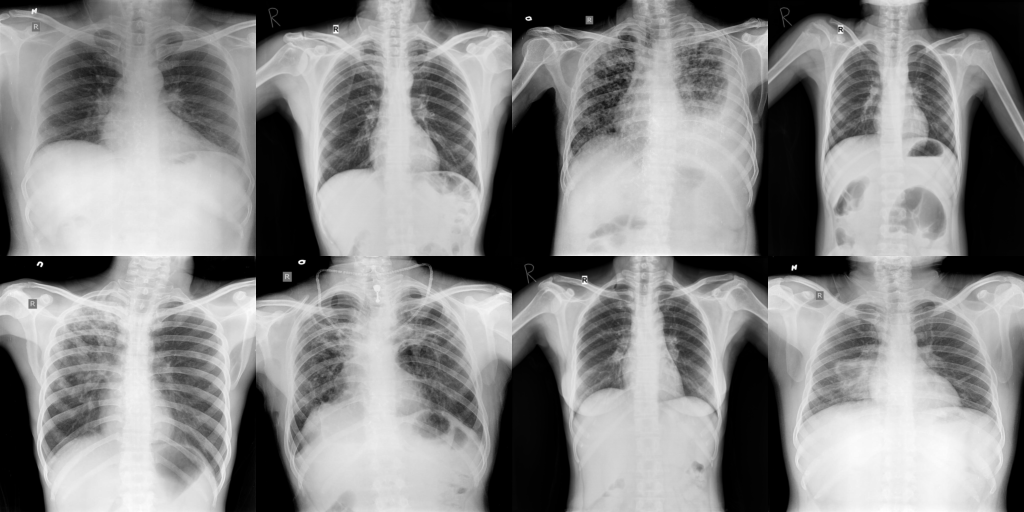
\includegraphics[height=0.25\textheight]{da-db-healthy.png}}
		%		\hfill
		\vfill
		%		\hfill
		\subcaptionbox{Пациенты, больные туберкулёзом лёгких}{%
			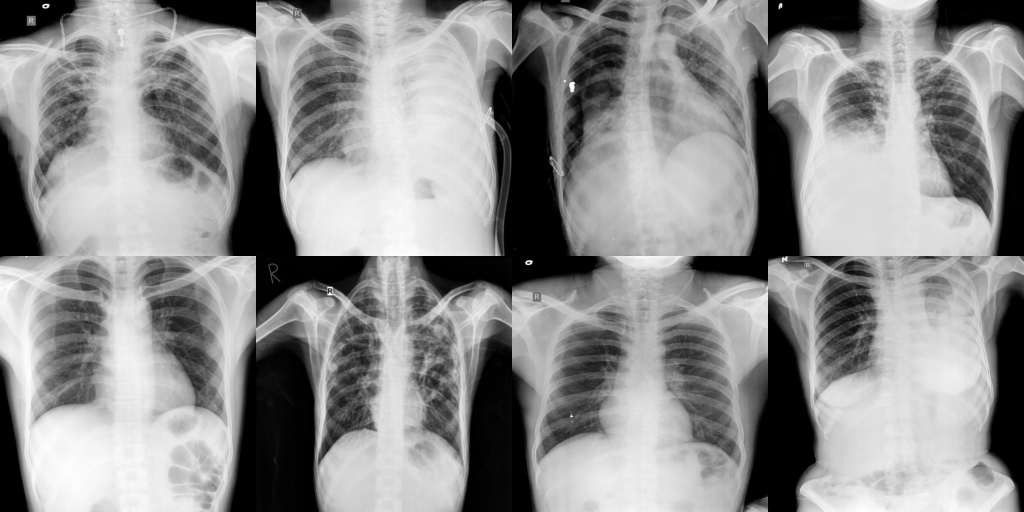
\includegraphics[height=0.25\textheight]{da-db-tb.png}}
		%		\hfill
		\vfill
	}
	\caption{Примеры изображений из объединённого набора DA~+~DB}
	\label{fig:samples-da-db}
\end{figure}

Фактическое количество изображений лёгких здоровых пациентов (далее "--- класс <<Healthy>>) и изображений лёгких пациентов с проявлениями туберкулёза (класс <<TB>>), для которых имеются метки классов, в использованных открытых наборах представлены в Табл.~\ref{tab:total-cxr}.

\begin{table} [htbp]%
	\centering
	\caption{Размеры рассматриваемых открытых наборов рентгенограмм грудной клетки}%
	\label{tab:total-cxr}% label всегда желательно идти после caption
	\renewcommand{\arraystretch}{1.5}%% Увеличение расстояния между рядами, для улучшения восприятия.
	\begin{SingleSpace}
		\begin{tabulary}{\textwidth}{@{}@{\extracolsep{10pt}}lccC@{}} %Вертикальные полосы не используются принципиально, как и лишние горизонтальные (допускается по ГОСТ 2.105 пункт 4.4.5) % @{} позволяет прижиматься к краям
			\toprule     %%% верхняя линейка
			& \multicolumn{2}{@{}c@{}}{Число снимков по классам} & \\
			\cmidrule{2-3}
			Набор данных & TB & Healthy & Общее число снимков \\
			\midrule %%% тонкий разделитель. Отделяет названия столбцов. Обязателен по ГОСТ 2.105 пункт 4.4.5
			Montgomery County (MC)    & 58  & 80  & 138  \\
			Shenzhen (SZ)    & 336   & 326  & 662  \\
			DA    & 78   & 78  & 156  \\
			DB    & 47   & 75  & 122  \\
			TBX11K    & 800   & 3800  & 4600  \\
			\bottomrule %%% нижняя линейка
		\end{tabulary}%
	\end{SingleSpace}
\end{table}

\subsection{Набор рентгенограмм грудной клетки Sakha"~TB}

Сформированный в рамках исследования набор рентгенограмм грудной клетки, сделанных во фронтальной проекции, собран в результате сотрудничества с несколькими медицинскими учреждениями Республики Саха (Якутия); ниже он обозначен <<Sakha"~TB>>. Процедура формирования набора изображений из имеющихся коллекций рентгенограмм включала в себя:

\begin{itemize}
	\item удаление снимков, сделанных в боковой проекции;
	\item контроль правильности установленных значений <<Photometric Interpretation>> в файлах DICOM;
	\item удаление повторяющихся сессий;
	\item удаление пациентов с несколькими сессиями;% и различиями в диагнозе между сессиями;
	\item удаление персональной информации;
	\item удаление несовершеннолетних пациентов;
	\item а также некоторую балансировку соотношения полов и распределений возрастов и диагнозов.
\end{itemize}

В результате было отобрано 400 изображений здоровых и 400 изображений больных туберкулёзом лёгких пациентов, где каждому пациенту соответствует только 1 снимок. Для получения рентгенограмм использовались стационарные и переносные комплексы оборудования. В основном разрешение изображений примерно равно 3000x3000 пикселей, но часть снимков имеет меньший размер вплоть до около 2000x2000 пикселей. Большинство изображений имеет глубину цвета 16 бит, у остальных снимков она равна 8 битам.

Врачебная диагностика осуществлялась посредством независимого двойного чтения снимков с подтверждением диагноза <<туберкулёз>> специалистами НПЦ~<<Фтизиатрия>> им. Е.Н.~Андреева на основании клинико-лабораторных и микробиологических данных.

Примеры рентгенограмм из сформированного набора изображений представлены на Рис.~\ref{fig:samples-yak-2}. Сравнение распределений снимков по диагнозу, полу и возрасту полученного набора и набора MC~+~SZ (для наборов TBX11K, DA и DB такие данные недоступны) изображены на Рис.~\ref{fig:sex-distr}"~\ref{fig:age-distr-tb}. Сам набор изображений Sakha"~TB доступен для загрузки на странице по ссылке: \url{https://imaging.cs.msu.ru/en/research/TB/Sakha-TB}.

\begin{figure}[ht]
	\centerfloat{
		%		\hfill
		\subcaptionbox[List-of-Figures entry]{Здоровые пациенты}{%
			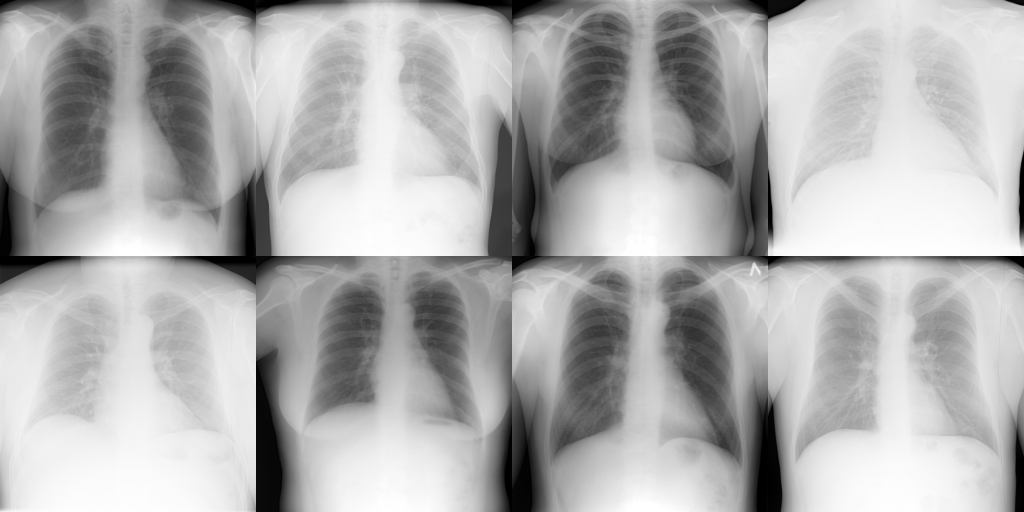
\includegraphics[height=0.25\textheight]{sakha-healthy.png}}
		%		\hfill
		\vfill
		%		\hfill
		\subcaptionbox{Пациенты, больные туберкулёзом лёгких}{%
			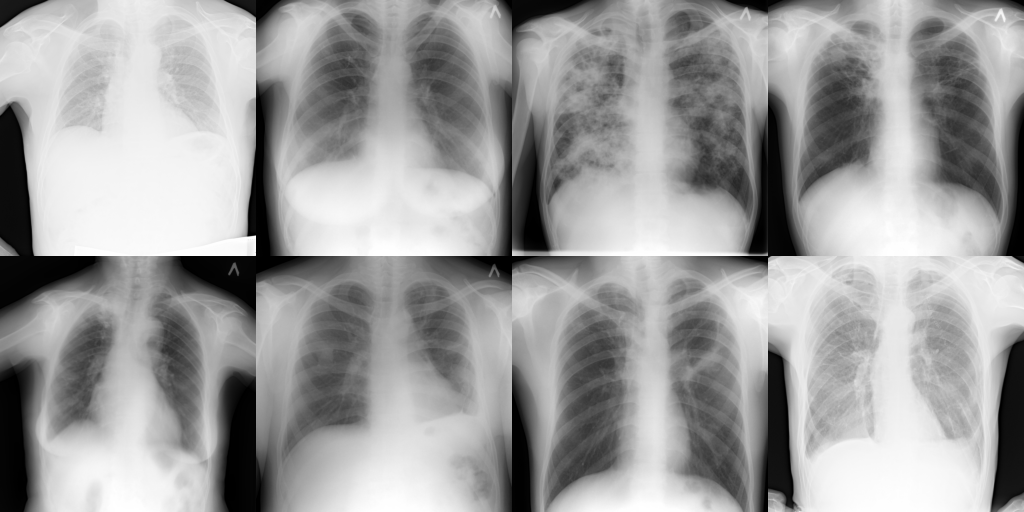
\includegraphics[height=0.25\textheight]{sakha-tb.png}}
		%		\hfill
		\vfill
	}
	\caption{Примеры изображений из набора Sakha"~TB}
	\label{fig:samples-yak-2}
\end{figure}

\begin{figure}[ht]
	\centerfloat{
		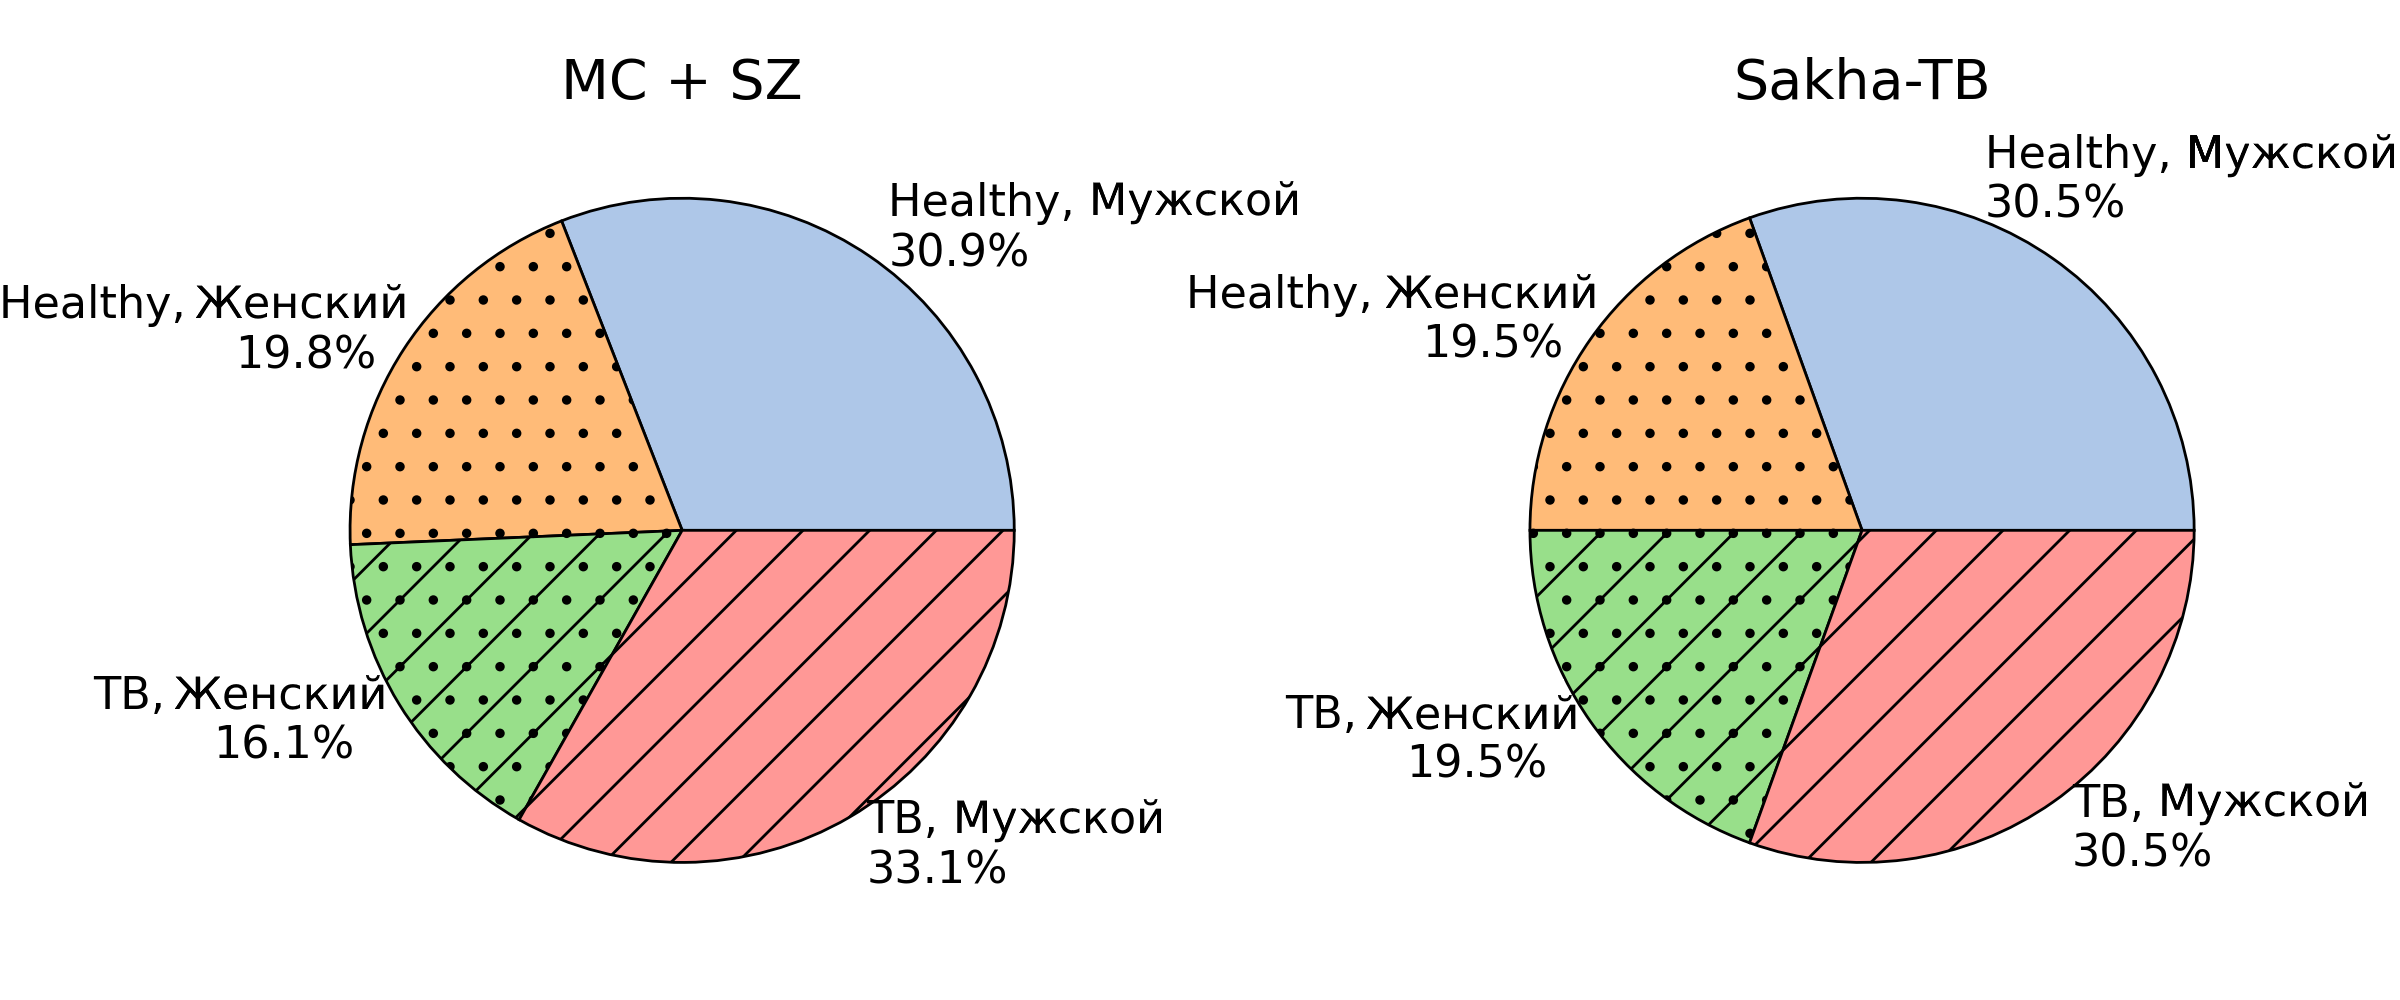
\includegraphics[width=0.9\textwidth]{diag-sex-distr-ru.png}
	}
	\caption{Распределение изображений в наборах MC~+~SZ и Sakha"~TB по диагнозу и полу}
	\label{fig:sex-distr}
\end{figure}

\begin{figure}[ht]
	\centerfloat{
		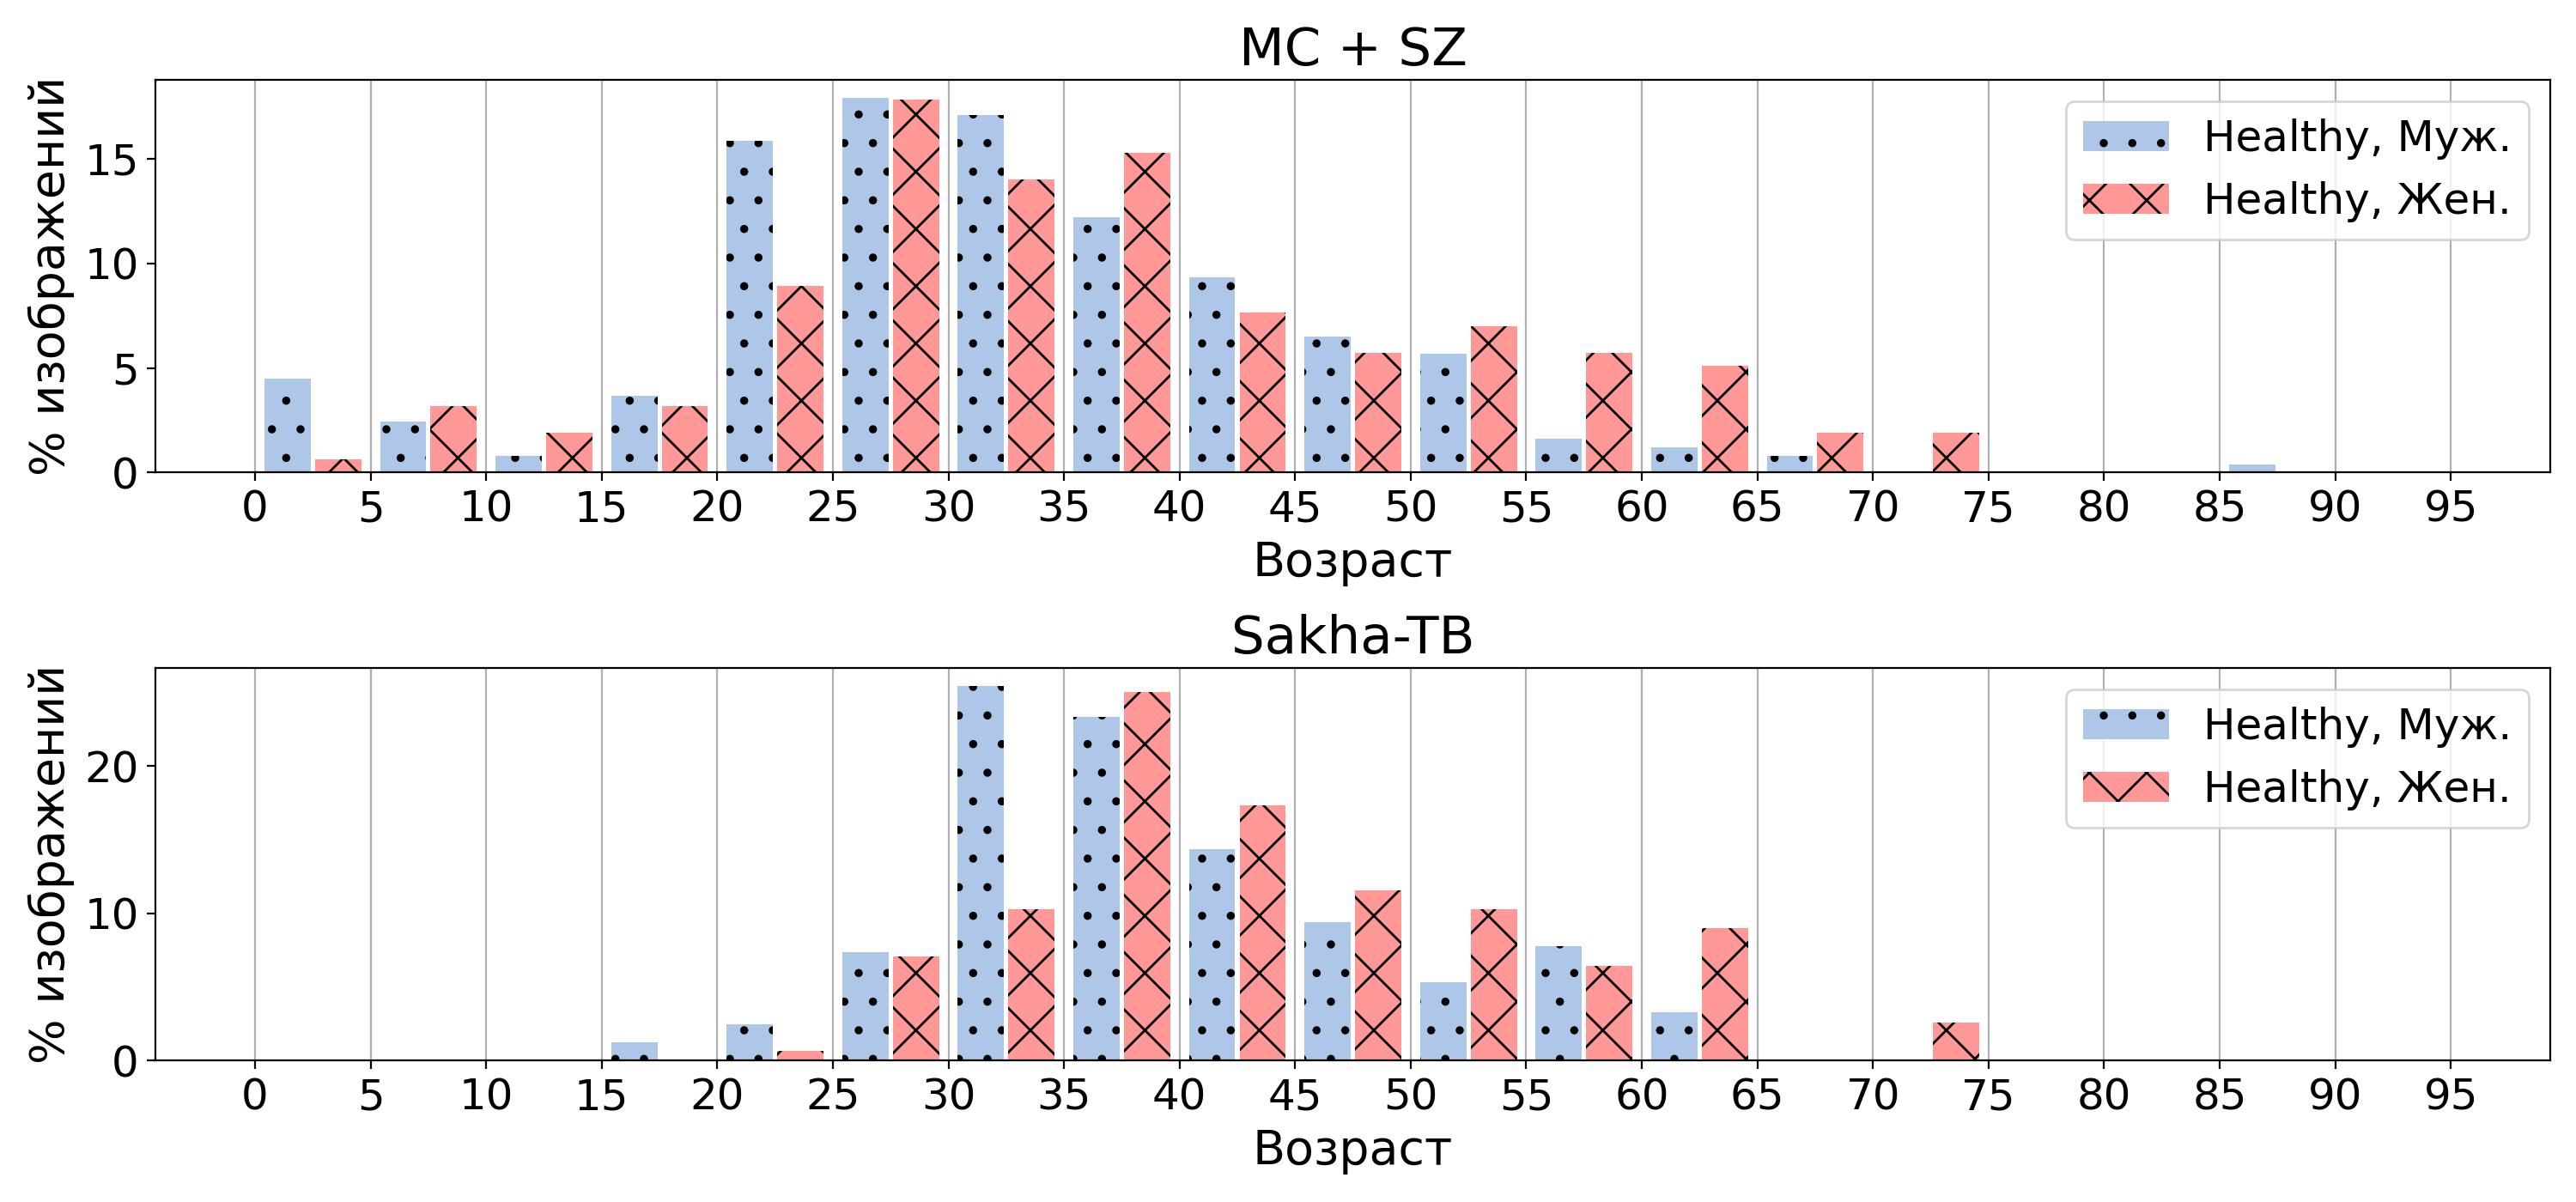
\includegraphics[width=0.9\textwidth]{sex-age-distr-healthy-ru.png}
	}
	\caption{Распределение изображений здоровых пациентов в наборах MC~+~SZ и Sakha"~TB по возрасту в зависимости от пола}
	\label{fig:age-distr-healthy}
\end{figure}

\begin{figure}[ht]
	\centerfloat{
		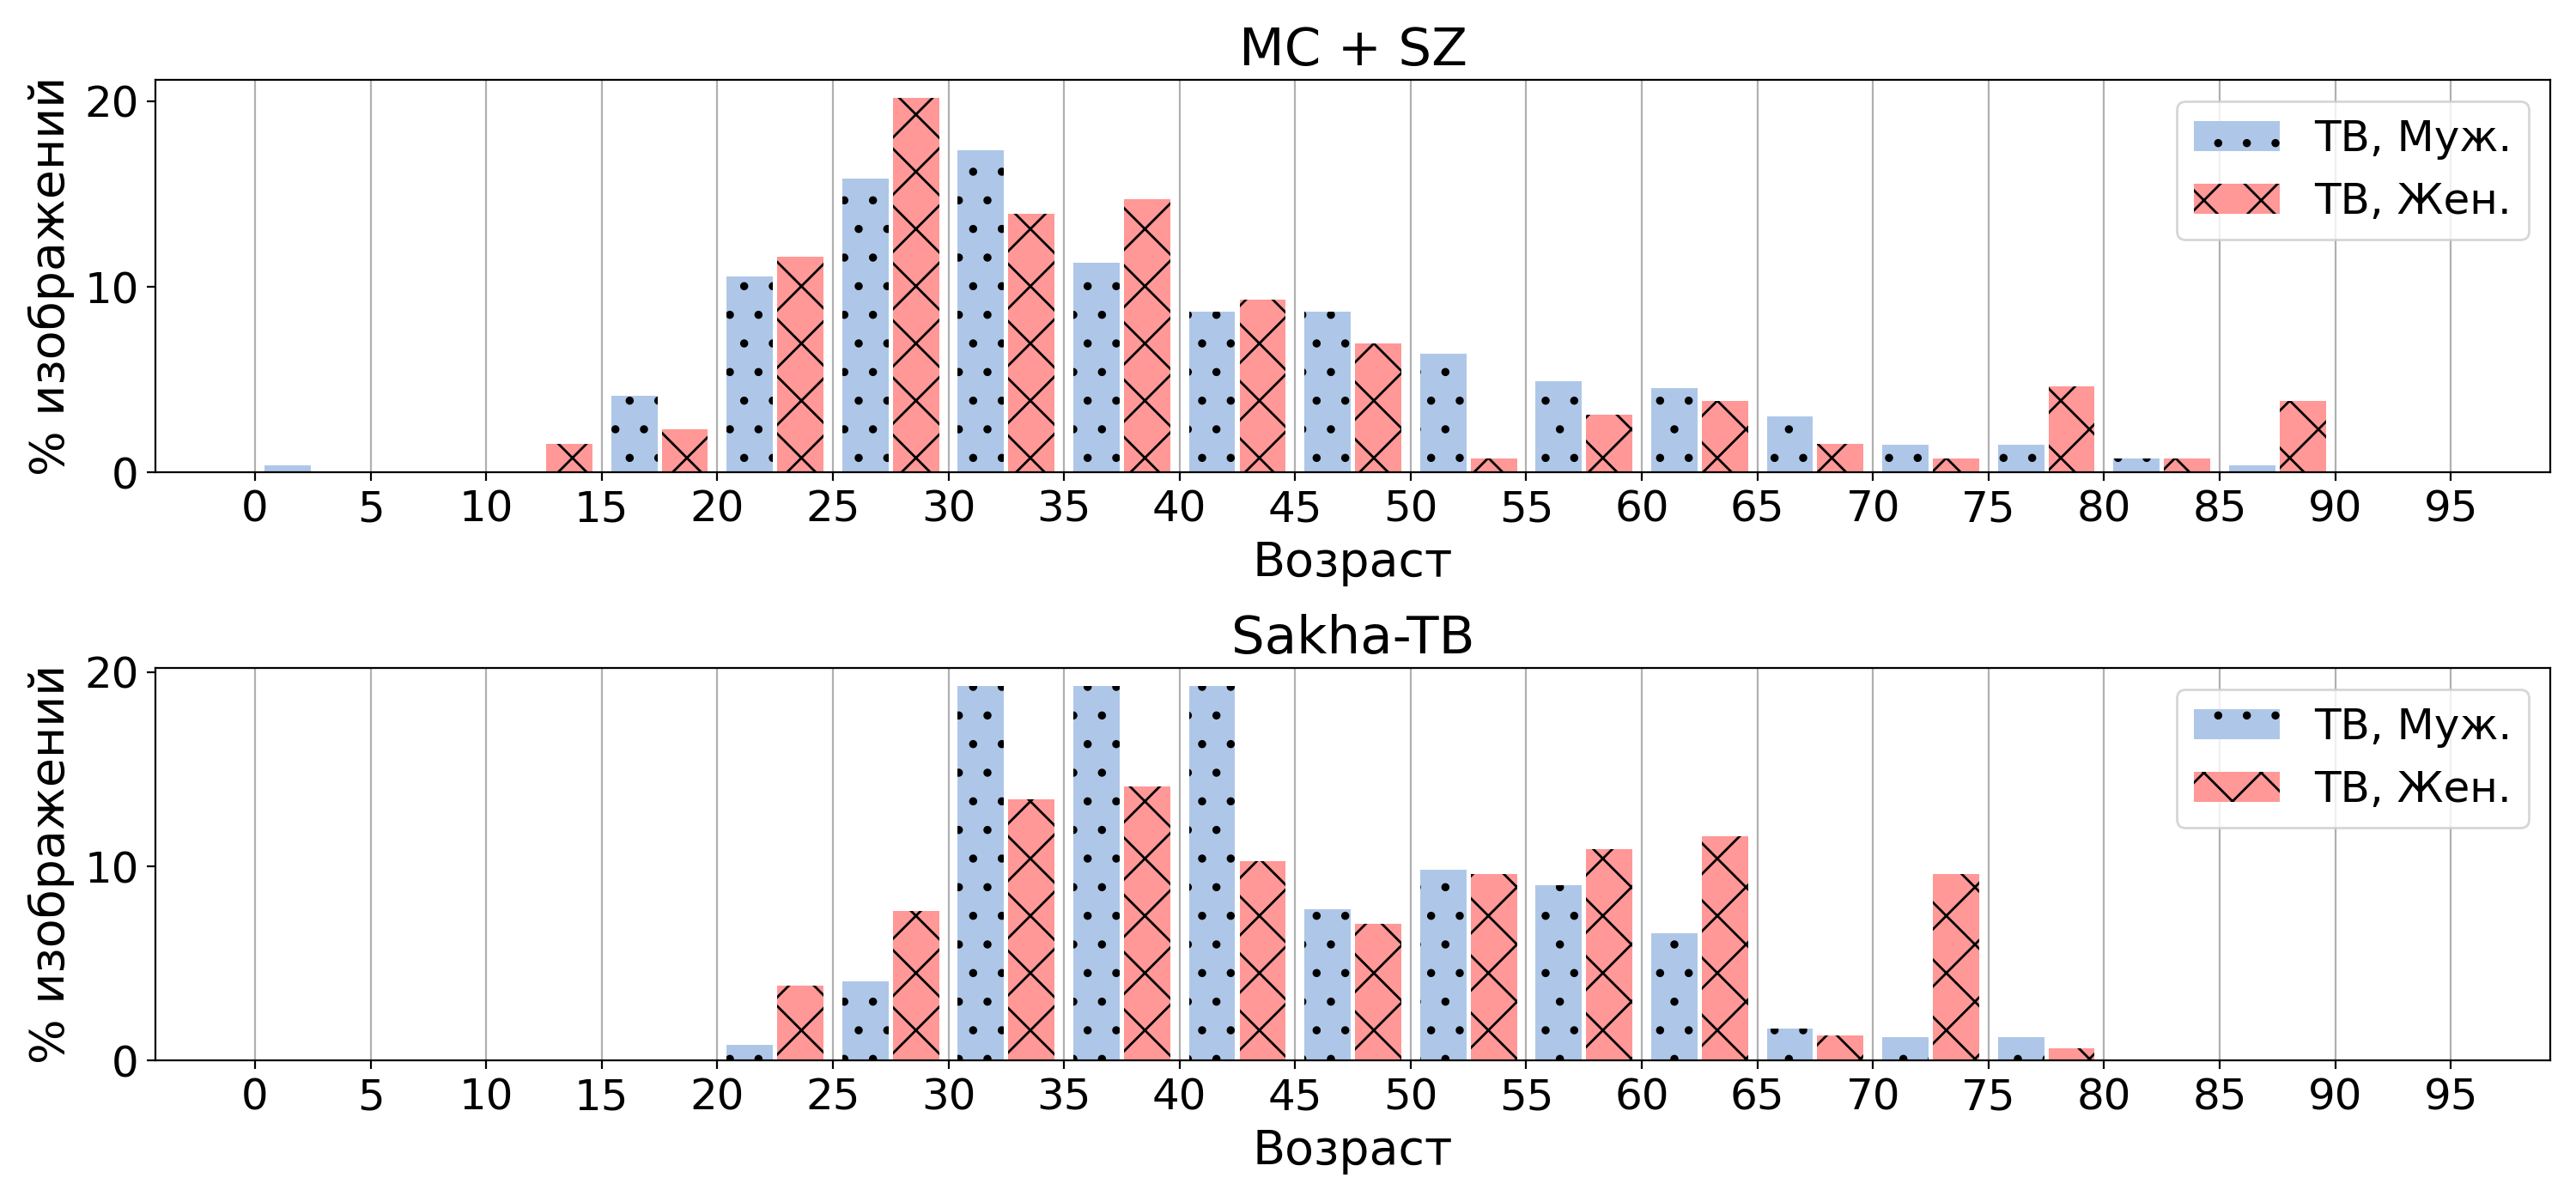
\includegraphics[width=0.9\textwidth]{sex-age-distr-tb-ru.png}
	}
	\caption{Распределение изображений больных туберкулёзом пациентов в наборах MC~+~SZ и Sakha"~TB по возрасту в зависимости от пола}
	\label{fig:age-distr-tb}
\end{figure}

\subsection{Эксперименты}

Для оценки возможностей применения предлагаемого набора изображений в задаче компьютерной диагностики туберкулёза были сделаны замеры качества работы методов глубокого обучения при обучении и тестировании на разных комбинациях рассматриваемых открытых наборов снимков:
\begin{enumerate}[beginpenalty=10000]
	\item MC~+~SZ,
	\item DA~+~DB,
	\item TBX11K,
	\item Sakha"~TB,
	\item (MC~+~SZ)~+~Sakh"~ TB,
	\item (DA~+~DB)~+~Sakha"~TB,
	\item TBX11K~+~Sakha"~TB,
	\item TBX11K~+~(MC~+~SZ),
	\item TBX11K~+~(MC~+~SZ)~+~(DA~+~DB),
	\item TBX11K~+~(MC~+~SZ)~+~(DA~+~DB)~+~Sakha"~TB.
\end{enumerate}

Снимки из набора Sakha"~TB предварительно подверглись обработке, совпадающей с описанной в п.~\ref{subsubsec:dataset-yak-hardness}.

Использованный в этом разделе для экспериментов алгоритм диагностики туберкулёза лёгких совпадал с описанным в п.~\ref{subsec:tbx-diagnostics}, за исключением следующих деталей.

В качестве основы нейросетевой модели были рассмотрены две современные модели EfficientNetV2"~M~\cite{tan2021efficientnetv2} и VisionTransformer"~Base/16~\cite{dosovitskiy2021an}, которые демонстрируют высокую точность в задачах классификации изображений. Далее варианты алгоритма на их основе будут обозначаться <<EffNetV2"~M>> и <<ViT"~B16>> соответственно. 

Размер пакета изображений составлял 64 для модели EffNetV2"~M и 32 для ViT"~B16. В конце каждой эпохи качество модели замерялось на валидационной выборке, при отсутствии уменьшения значения функции потерь на ней в течение 5 эпох шаг градиентного спуска уменьшался в 5 раз. Для предотвращения переобучения при отсутствии уменьшения значения функции потерь на валидационной выборке в течение 16 эпох обучение прерывалось. В качестве финального состояния весов модели принималось значение весов, соответствующие эпохе с наивысшим значением показателя качества на валидационной выборке. %Графики зависимости функции потерь от номера эпохи в процессе обучения представлены на Рис.~\ref{fig:tbx-loss-mc-sz}-~\ref{fig:tbx-loss-sakha}.

%\begin{figure}[ht]%
%	\centering
%	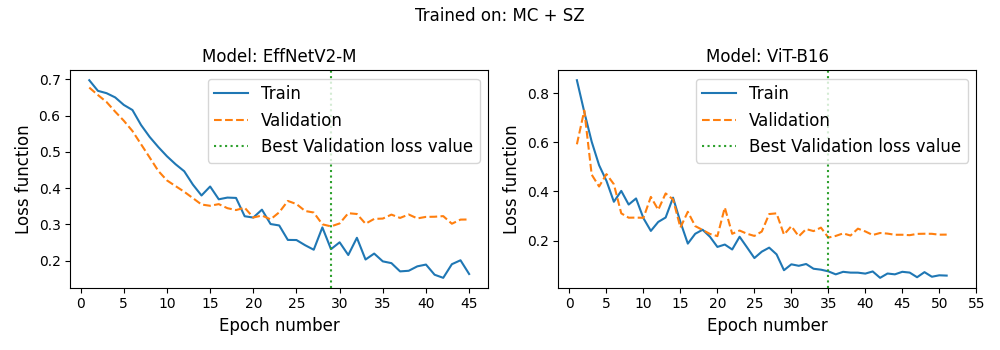
\includegraphics[width=0.9\textwidth]{loss-mc-sz-wide.png}
%	\caption{Графики зависимости функции потерь от номера эпохи для набора данных MC~+~SZ}\label{fig:tbx-loss-mc-sz}
%\end{figure}
%
%\begin{figure}[ht]%
%	\centering
%	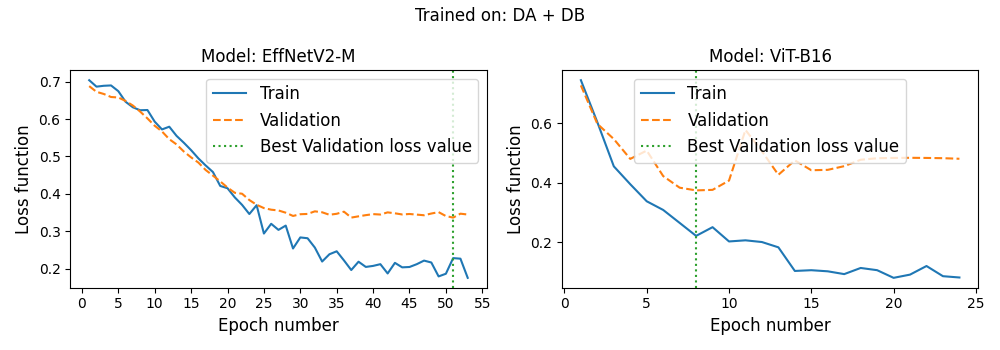
\includegraphics[width=0.9\textwidth]{loss-da-db-wide.png}
%	\caption{Графики зависимости функции потерь от номера эпохи для набора данных DA~+~DB}\label{fig:tbx-loss-da-db}
%\end{figure}
%
%\begin{figure}[ht]%
%	\centering
%	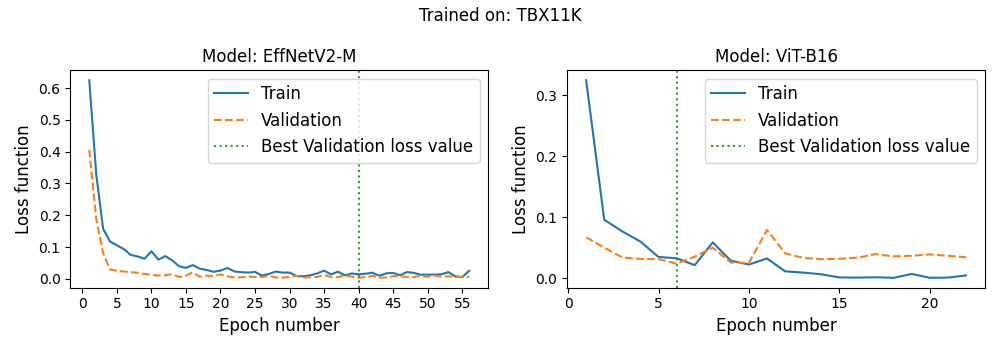
\includegraphics[width=0.9\textwidth]{loss-tbx11k-wide.png}
%	\caption{Графики зависимости функции потерь от номера эпохи для набора данных TBX11K}\label{fig:tbx-loss-tbx11k}
%\end{figure}
%
%\begin{figure}[ht]%
%	\centering
%	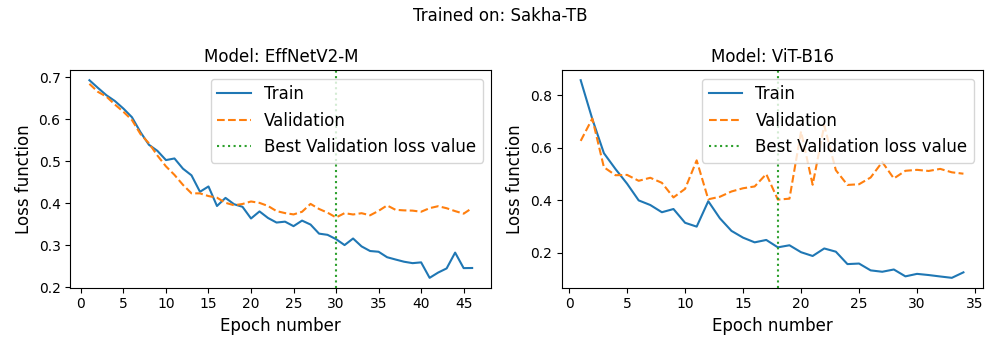
\includegraphics[width=0.9\textwidth]{loss-sakha-wide.png}
%	\caption{Графики зависимости функции потерь от номера эпохи для набора данных Sakha"~TB}\label{fig:tbx-loss-sakha}
%\end{figure}

\subsection{Результаты}
Замеры качества работы обученных алгоритмов на рассматриваемых наборах производились с использованием статистических показателей чувствительности (англ.~sensitivity) и специфичности (англ.~specificity), широко применяемых в медицине. Были построены ROC"~кривые, которые позволяют оценить общие возможности алгоритма классификации с учётом возможности варьирования порога уверенности для каждого класса. Интегральным показателем возможностей алгоритма в таком случае может считаться величина ROC~AUC, представляющая собой площадь под ROC"~кривой рассматриваемого алгоритма, которая принимает значения от 0 до 1, где 1 соответствует абсолютно точному алгоритму. ROC"~кривые с показателями ROC~AUC для рассмотренных моделей, обученных на некоторых из приведённых выше комбинаций рассматриваемых наборов рентгеновских снимков грудной клетки, представлены на Рис.~
%\ref{fig-roc-mc-sz}--\ref{fig-roc-tbx11k-mc-sz-da-db-sakha}.
\ref{fig-roc-mc-sz}--\ref{fig-roc-tbx11k-sakha}.
Для построения кривых для наборов, вошедших в обучающую выборку алгоритма, использовались их тестовые выборки, такие наборы выделены звёздочкой в описании графика; в противном случае использовались все наборы целиком.

\begin{figure}[ht]%
	\centering
	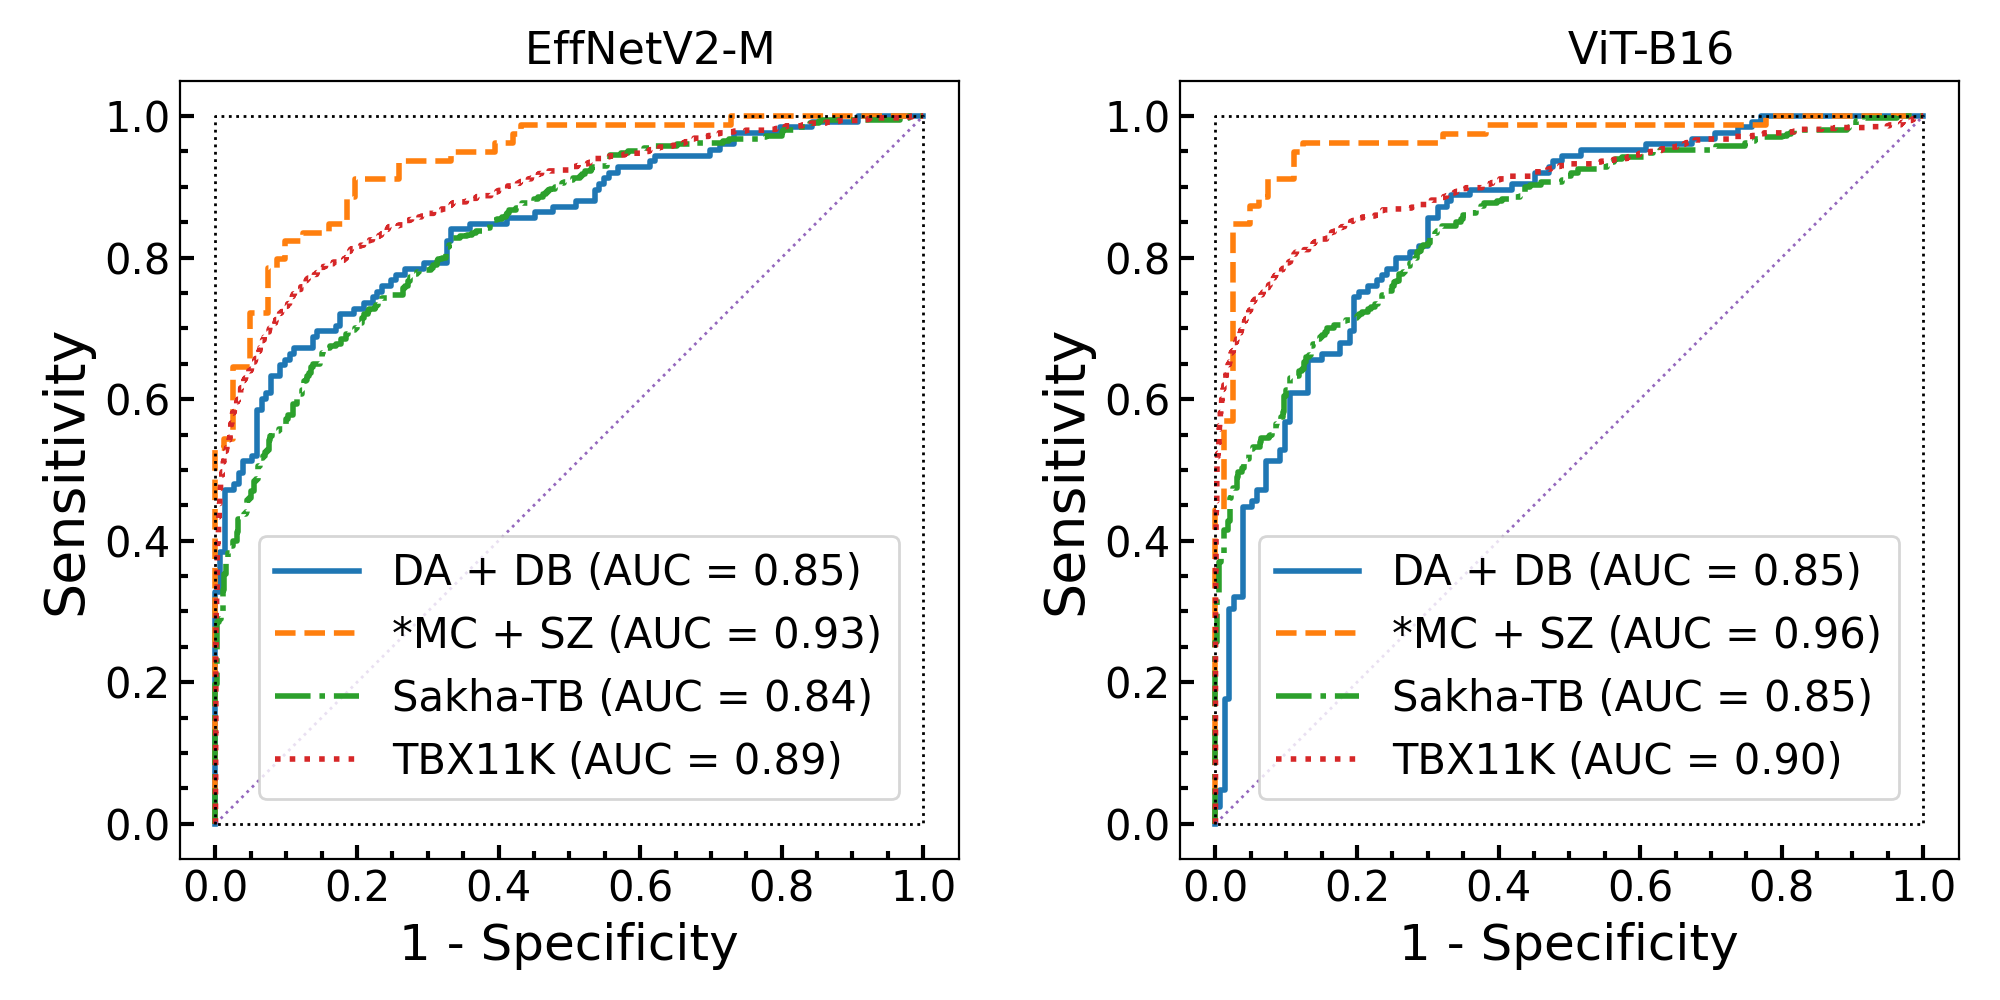
\includegraphics[width=0.9\textwidth]{roc-mc-sz-ru.png}
	\caption{Графики ROC"~кривых для моделей, обученных на наборе MC~+~SZ}\label{fig-roc-mc-sz}
\end{figure}
%
%\begin{figure}[ht]%
%	\centering
%	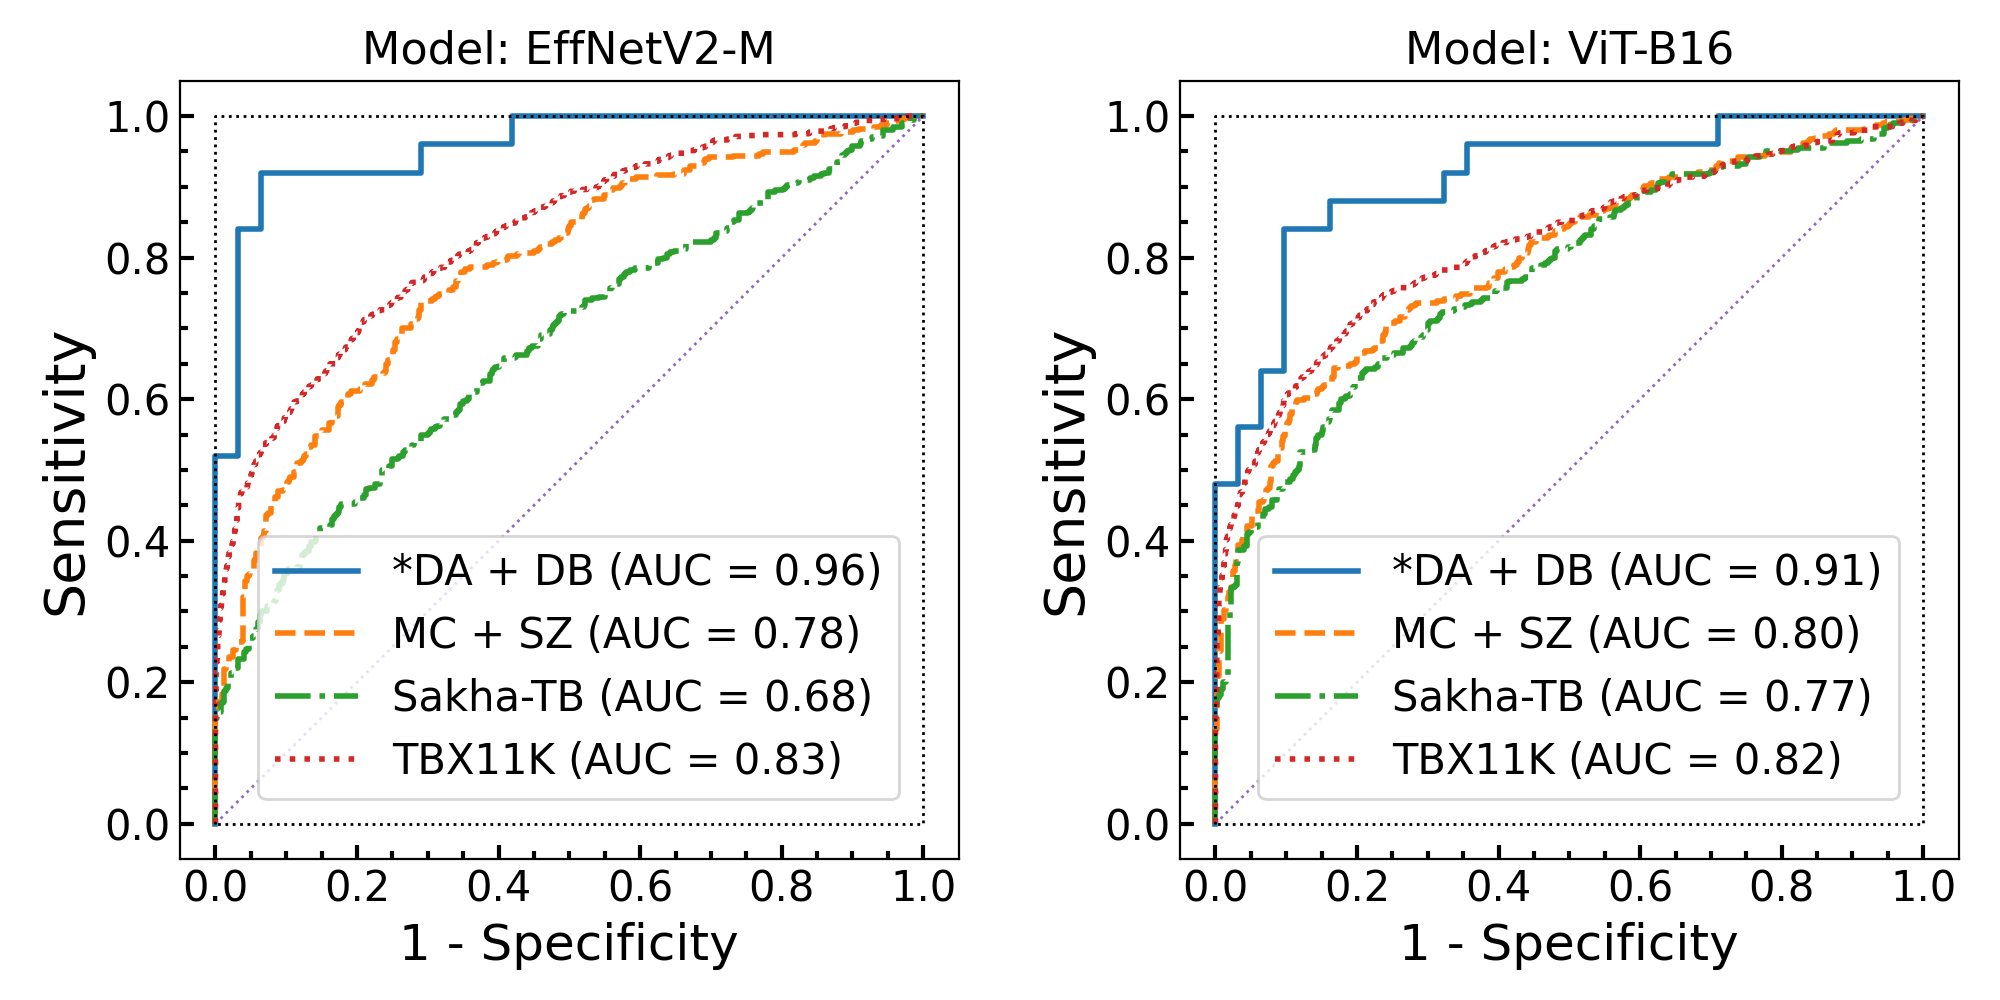
\includegraphics[width=0.9\textwidth]{roc-da-db.png}
%	\caption{Графики ROC"~кривых для моделей, обученных на наборе DA~+~DB}\label{fig-roc-da-db}
%\end{figure}
%
\begin{figure}[ht]%
	\centering
	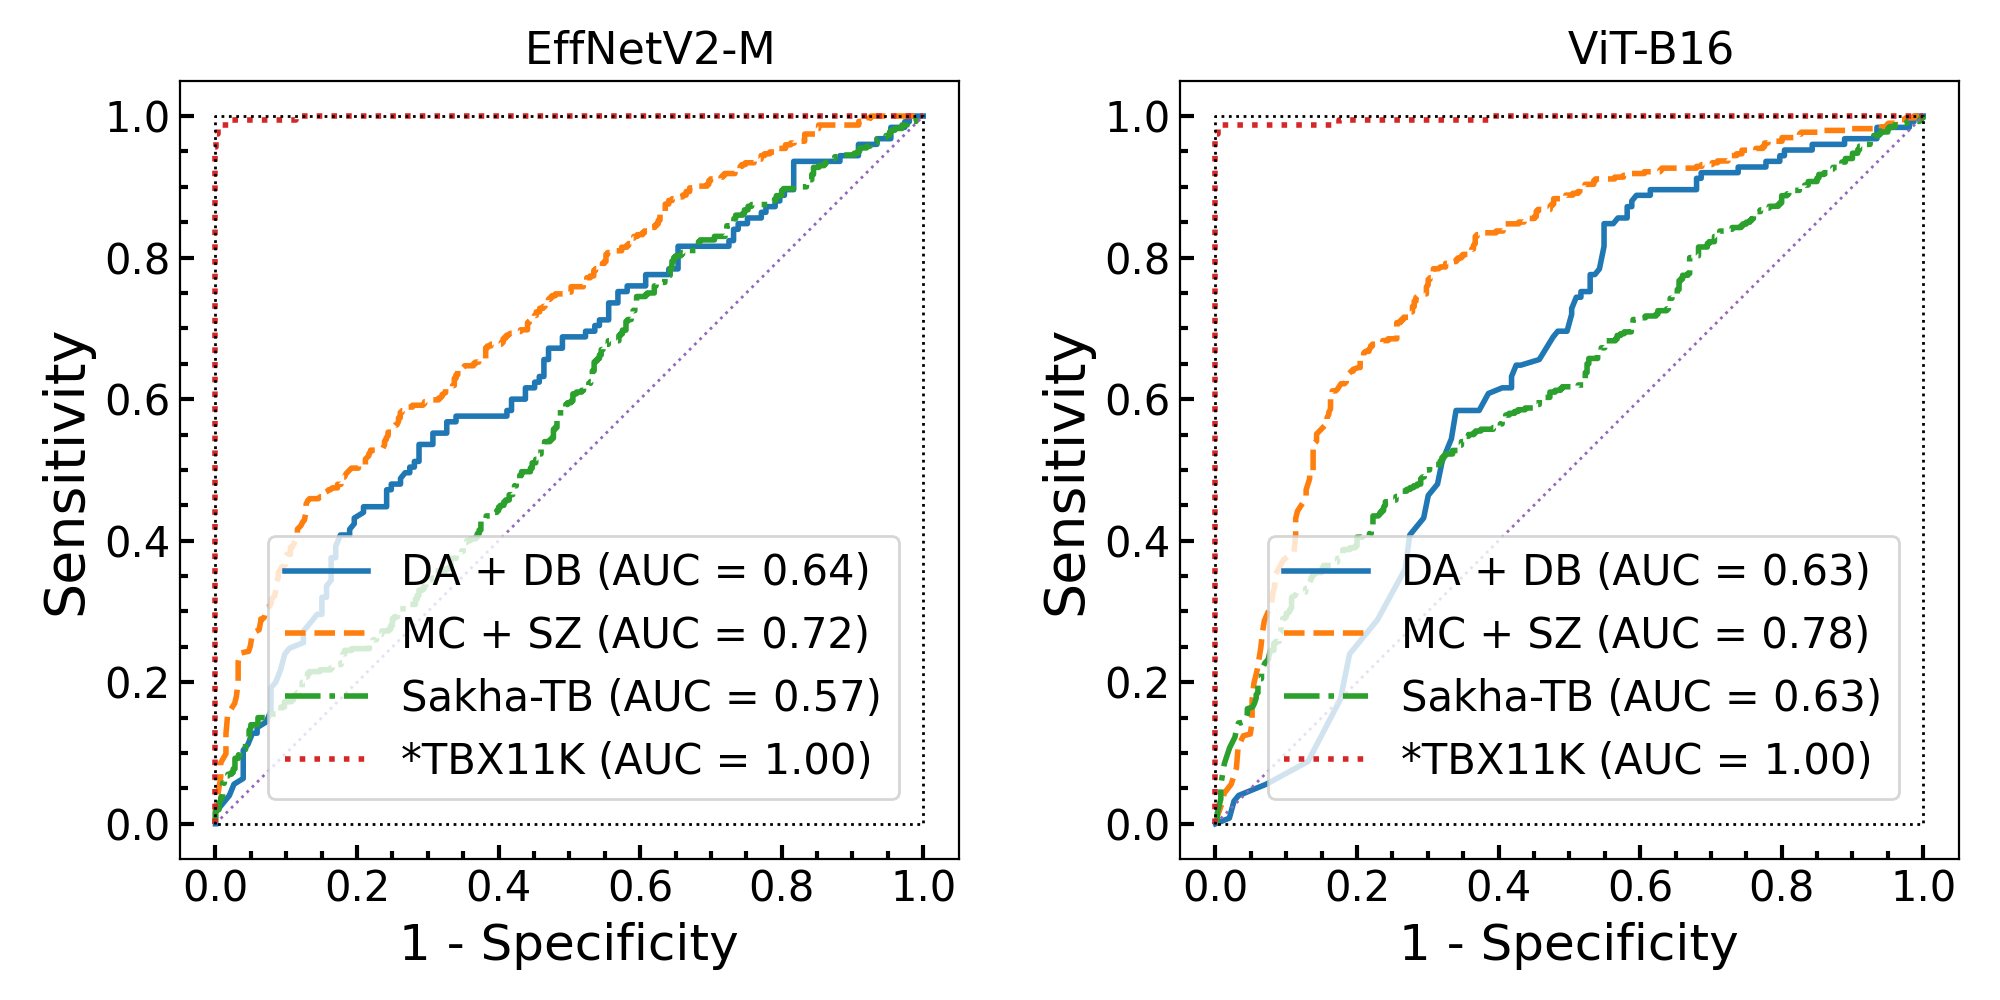
\includegraphics[width=0.9\textwidth]{roc-tbx11k-ru.png}
	\caption{Графики ROC"~кривых для моделей, обученных на наборе TBX11K}\label{fig-roc-tbx11k}
\end{figure}

%\begin{figure}[ht]%
%	\centering
%	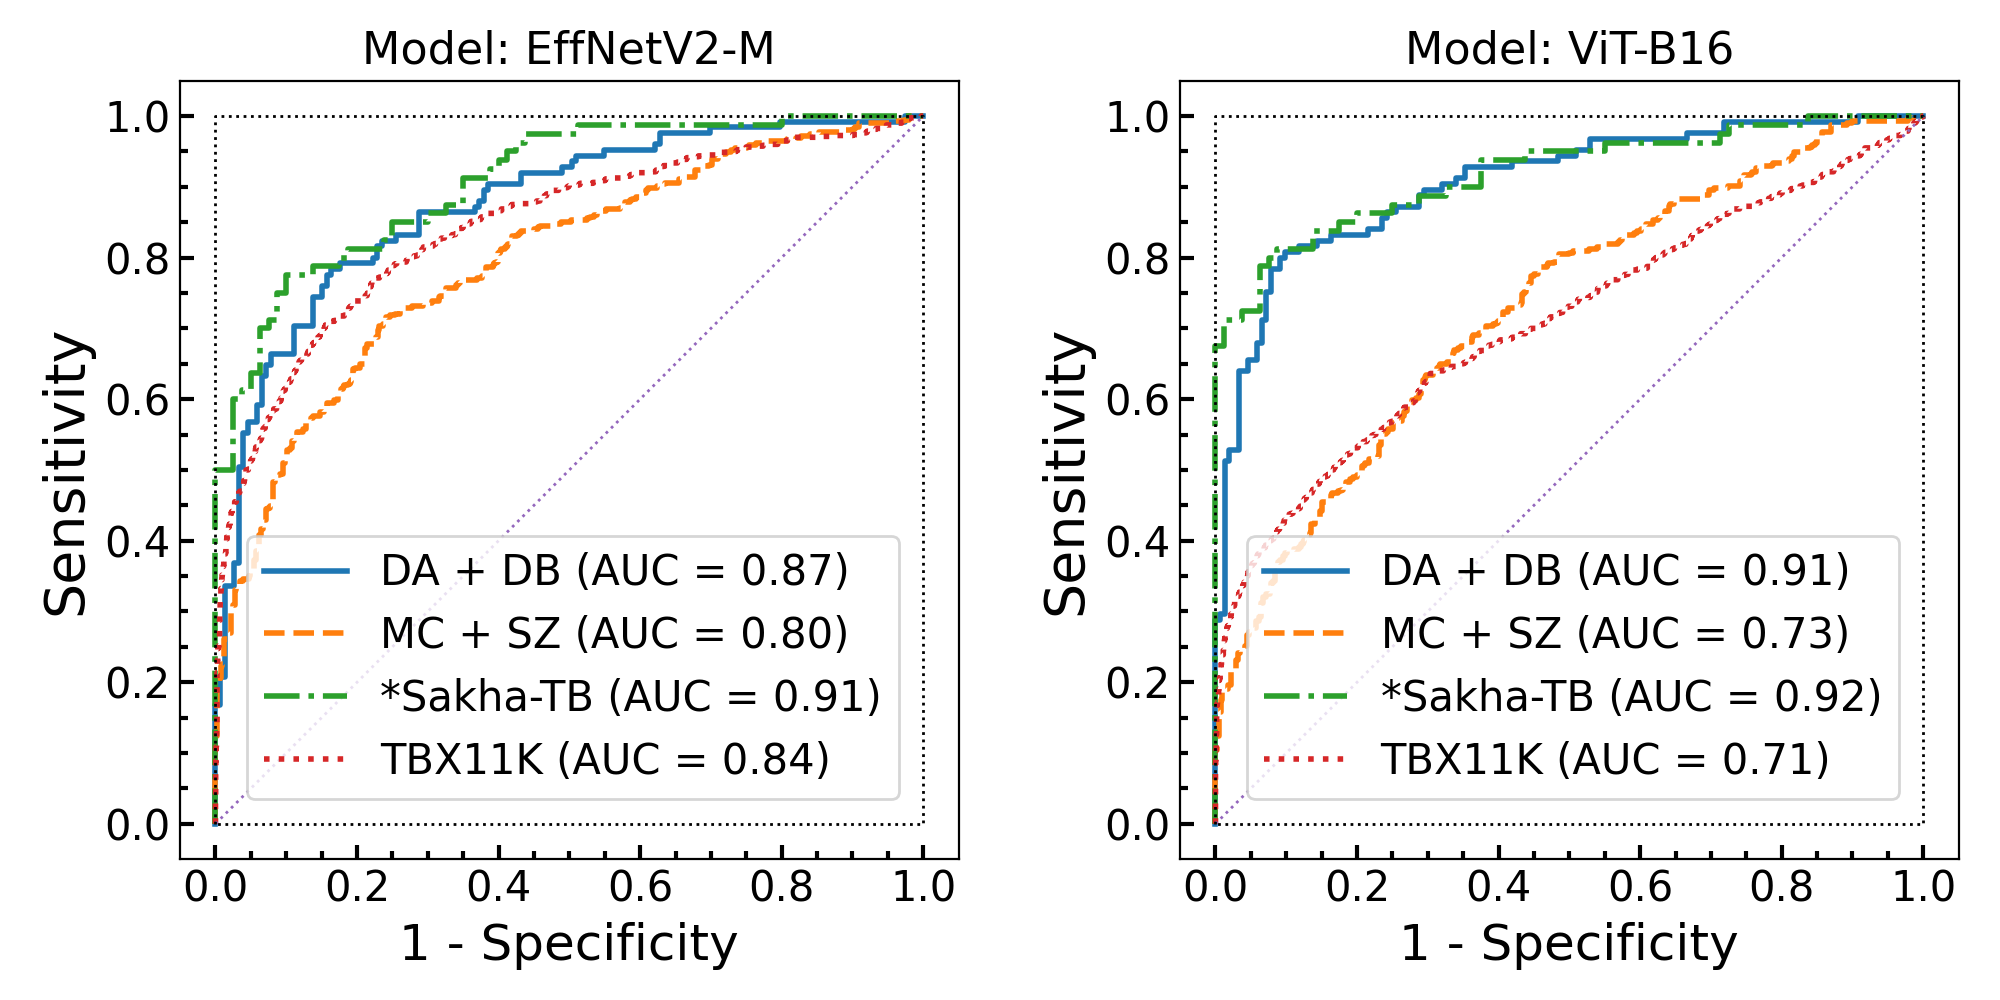
\includegraphics[width=0.9\textwidth]{roc-sakha.png}
%	\caption{Графики ROC"~кривых для моделей, обученных на наборе Sakha"~TB}\label{fig-roc-sakha}
%\end{figure}

\begin{figure}[ht]%
	\centering
	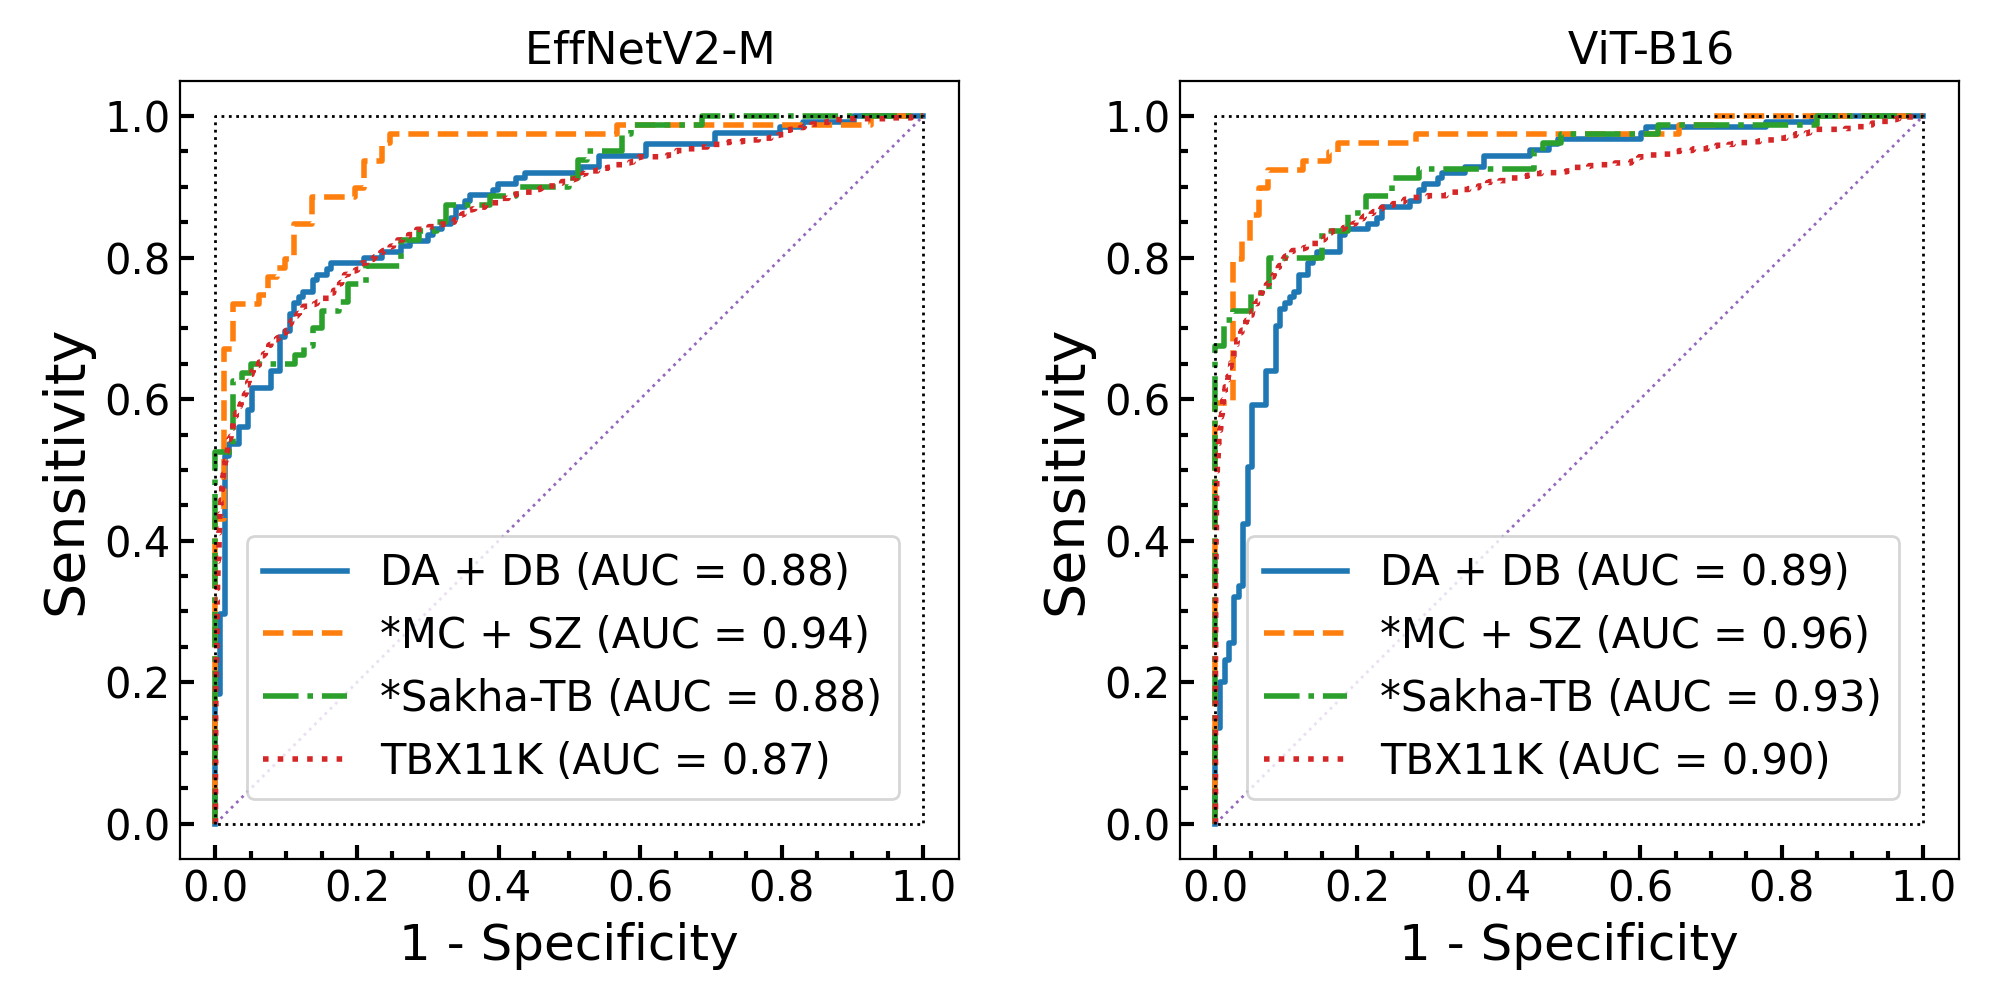
\includegraphics[width=0.9\textwidth]{roc-sakha-mc-sz-ru.png}
	\caption{Графики ROC"~кривых для моделей, обученных на наборе (MC~+~SZ)~+~Sakha"~TB}\label{fig-roc-mc-sz-sakha}
\end{figure}

%\begin{figure}[ht]%
%	\centering
%	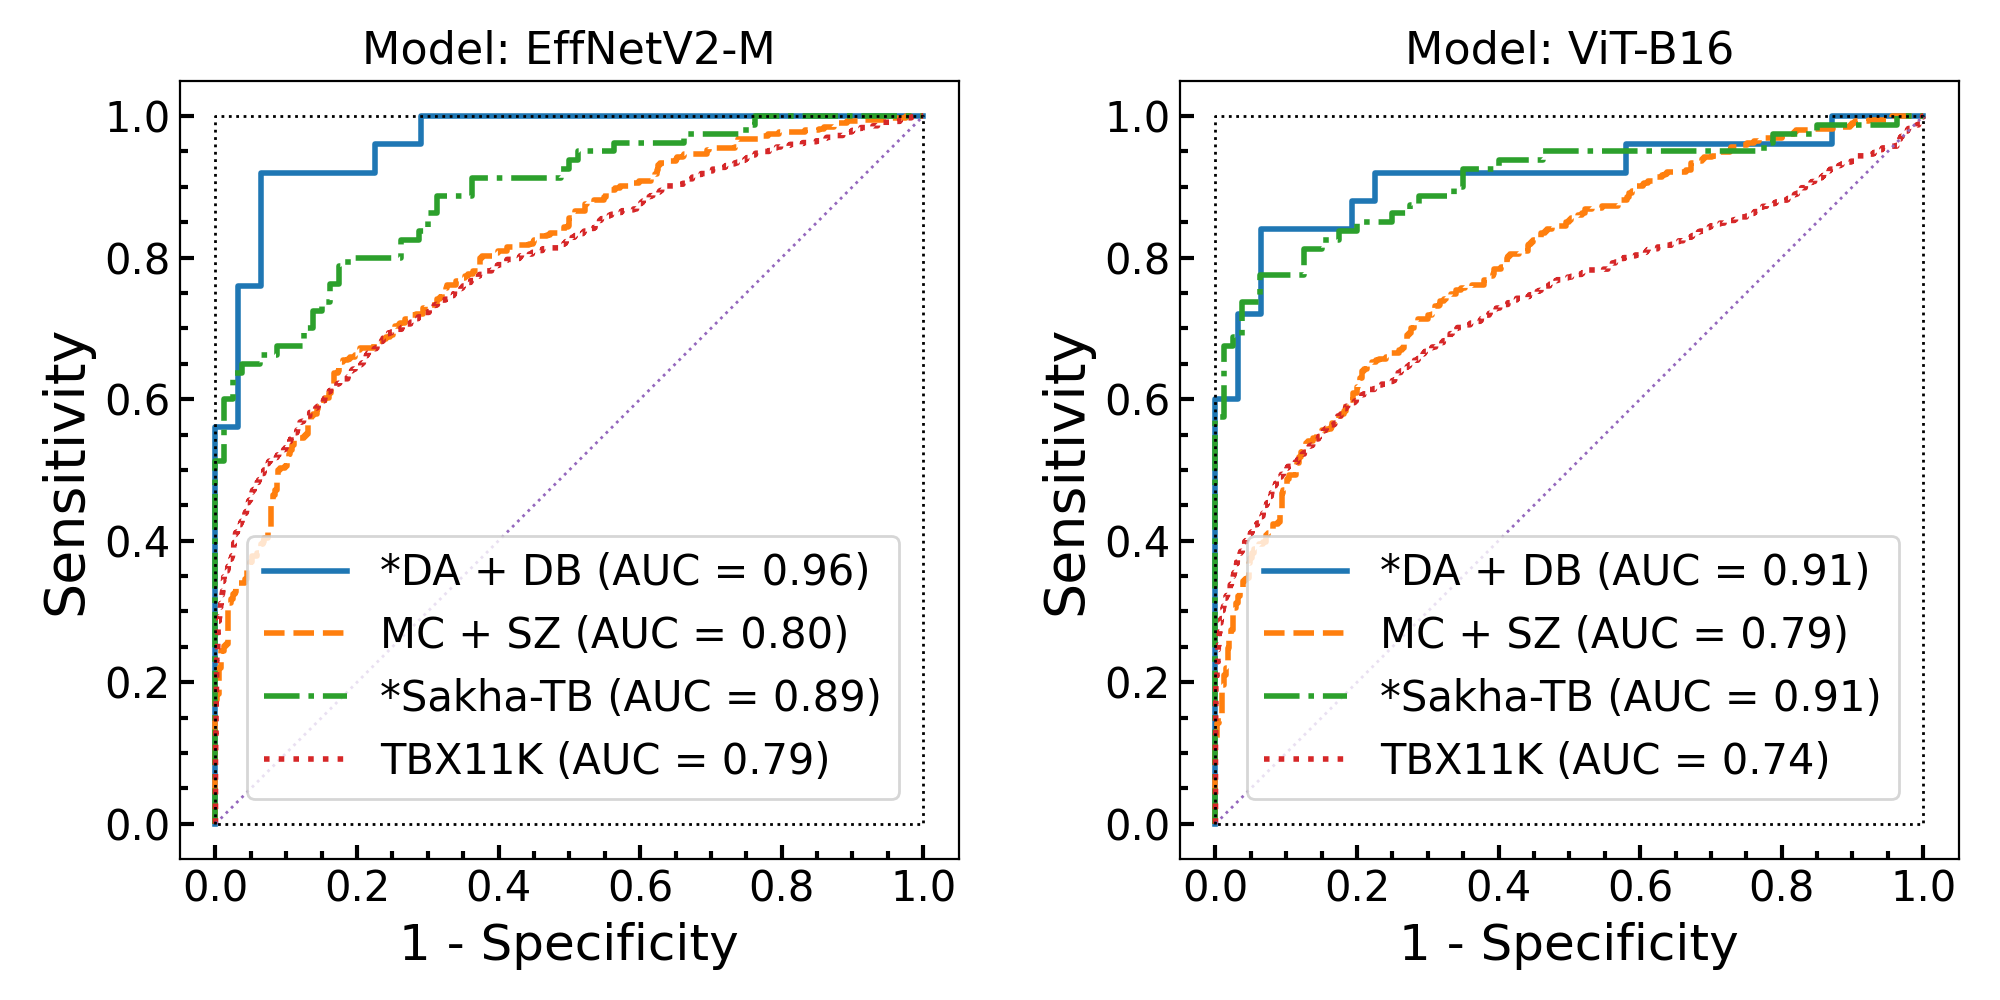
\includegraphics[width=0.9\textwidth]{roc-sakha-da-db.png}
%	\caption{Графики ROC"~кривых для моделей, обученных на наборе (DA~+~DB)~+~Sakha"~TB}\label{fig-roc-da-db-sakha}
%\end{figure}

\begin{figure}[ht]%
	\centering
	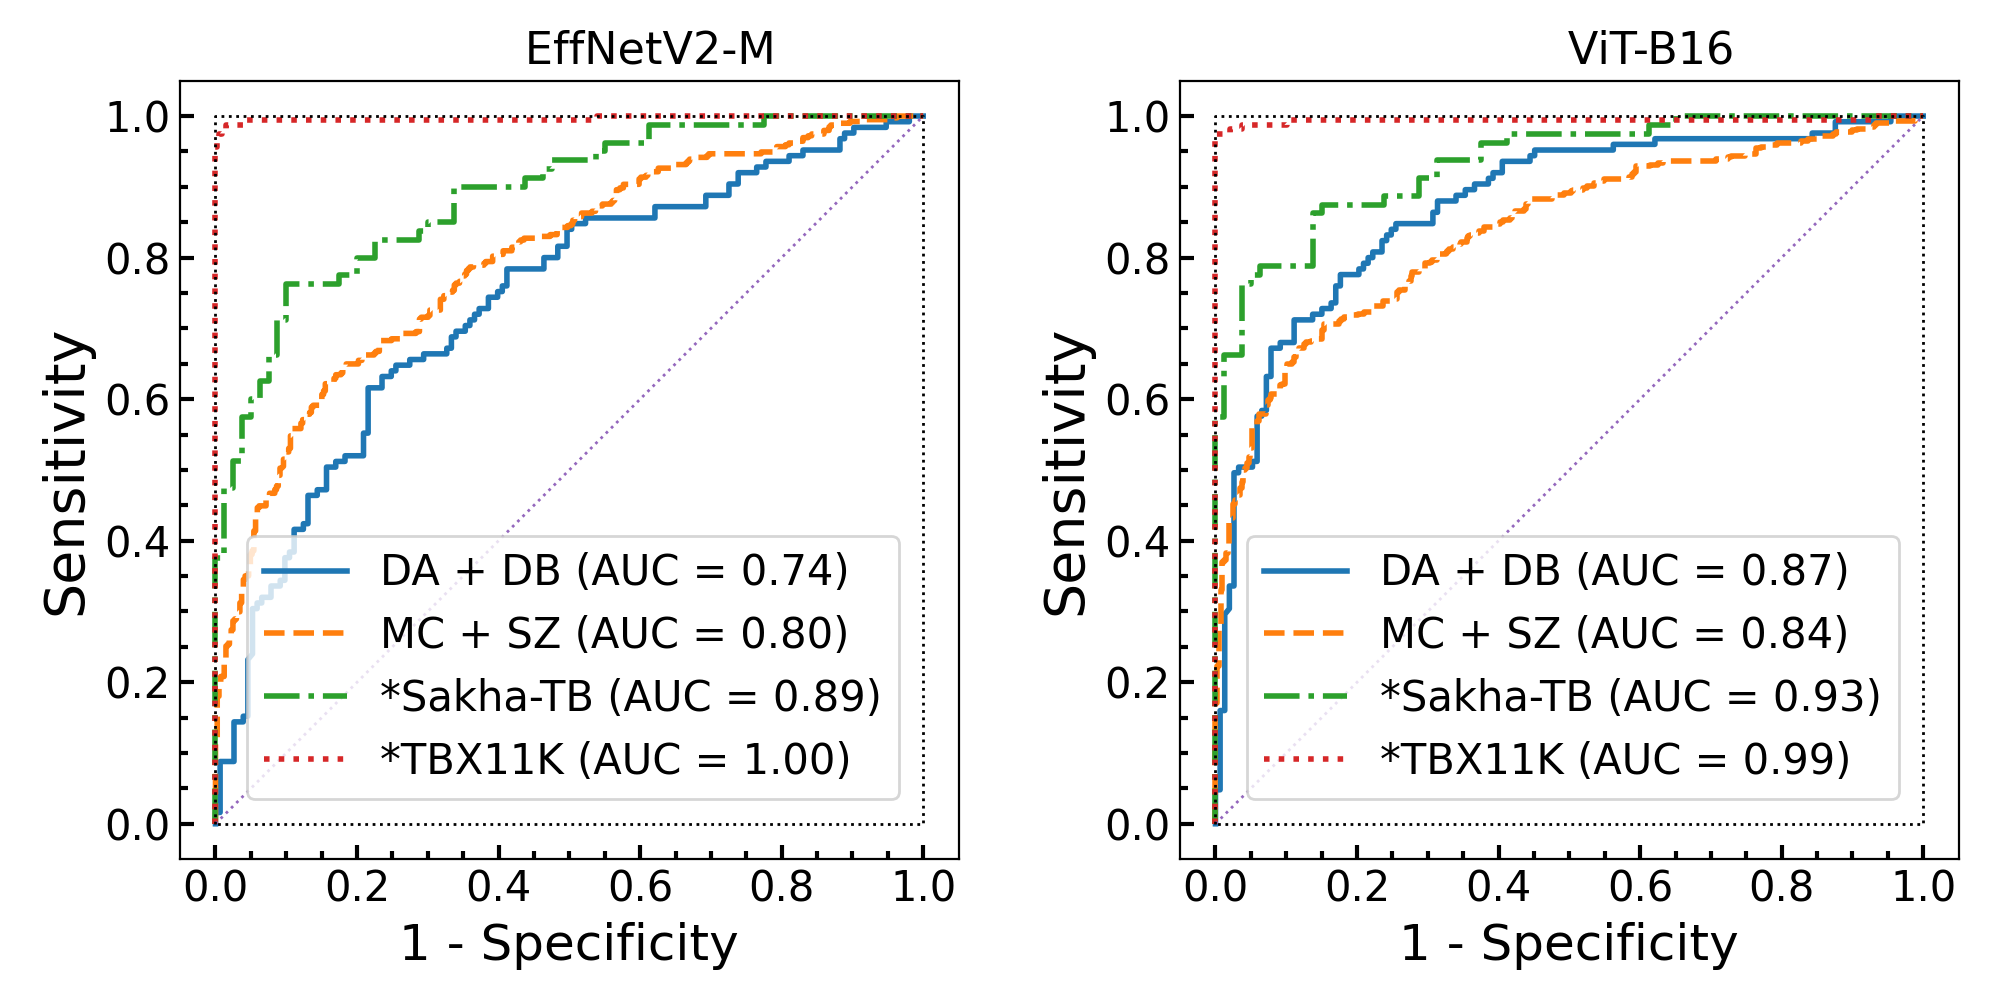
\includegraphics[width=0.9\textwidth]{roc-sakha-tbx11k-ru.png}
	\caption{Графики ROC"~кривых для моделей, обученных на наборе TBX11K~+~Sakha"~TB}\label{fig-roc-tbx11k-sakha}
\end{figure}

%\begin{figure}[ht]%
%	\centering
%	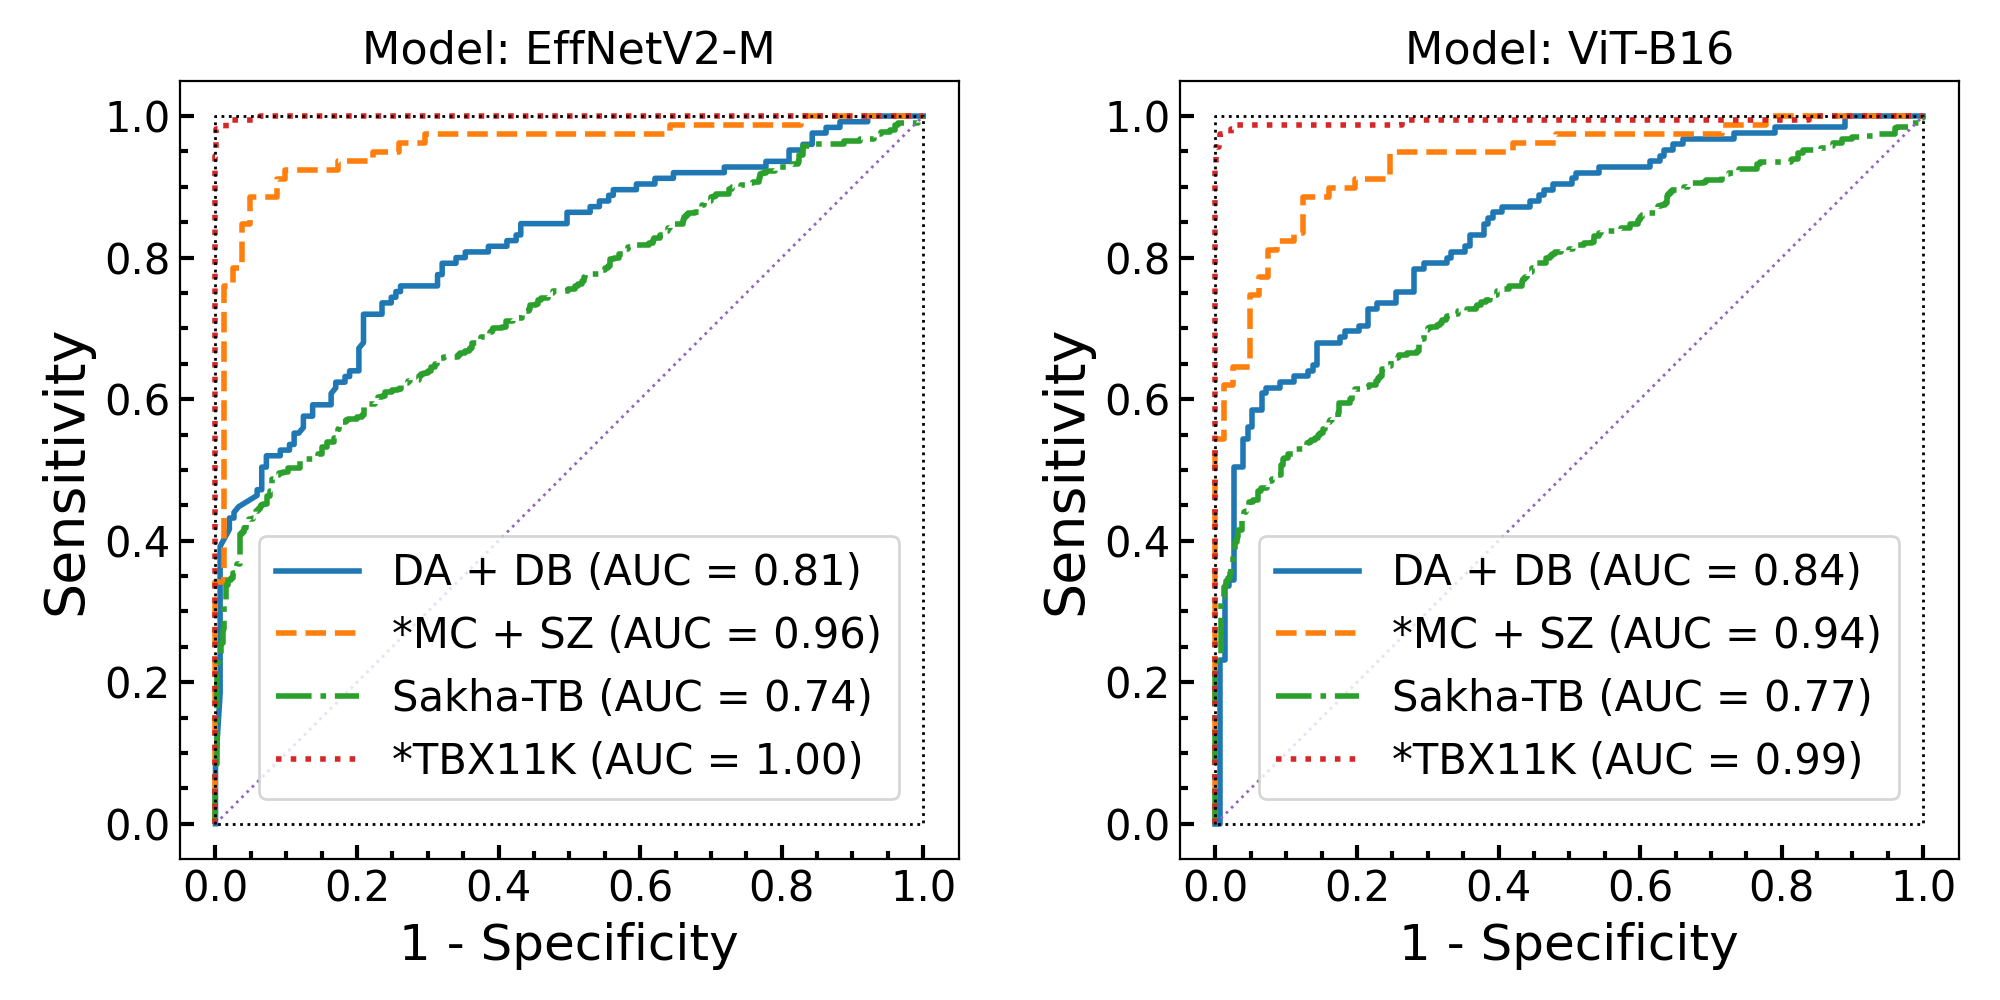
\includegraphics[width=0.9\textwidth]{roc-tbx11k-mc-sz.png}
%	\caption{Графики ROC"~кривых для моделей, обученных на наборе TBX11K~+~(MC~+~SZ)}\label{fig-roc-tbx11k-mc-sz}
%\end{figure}

%\begin{figure}[ht]%
%	\centering
%	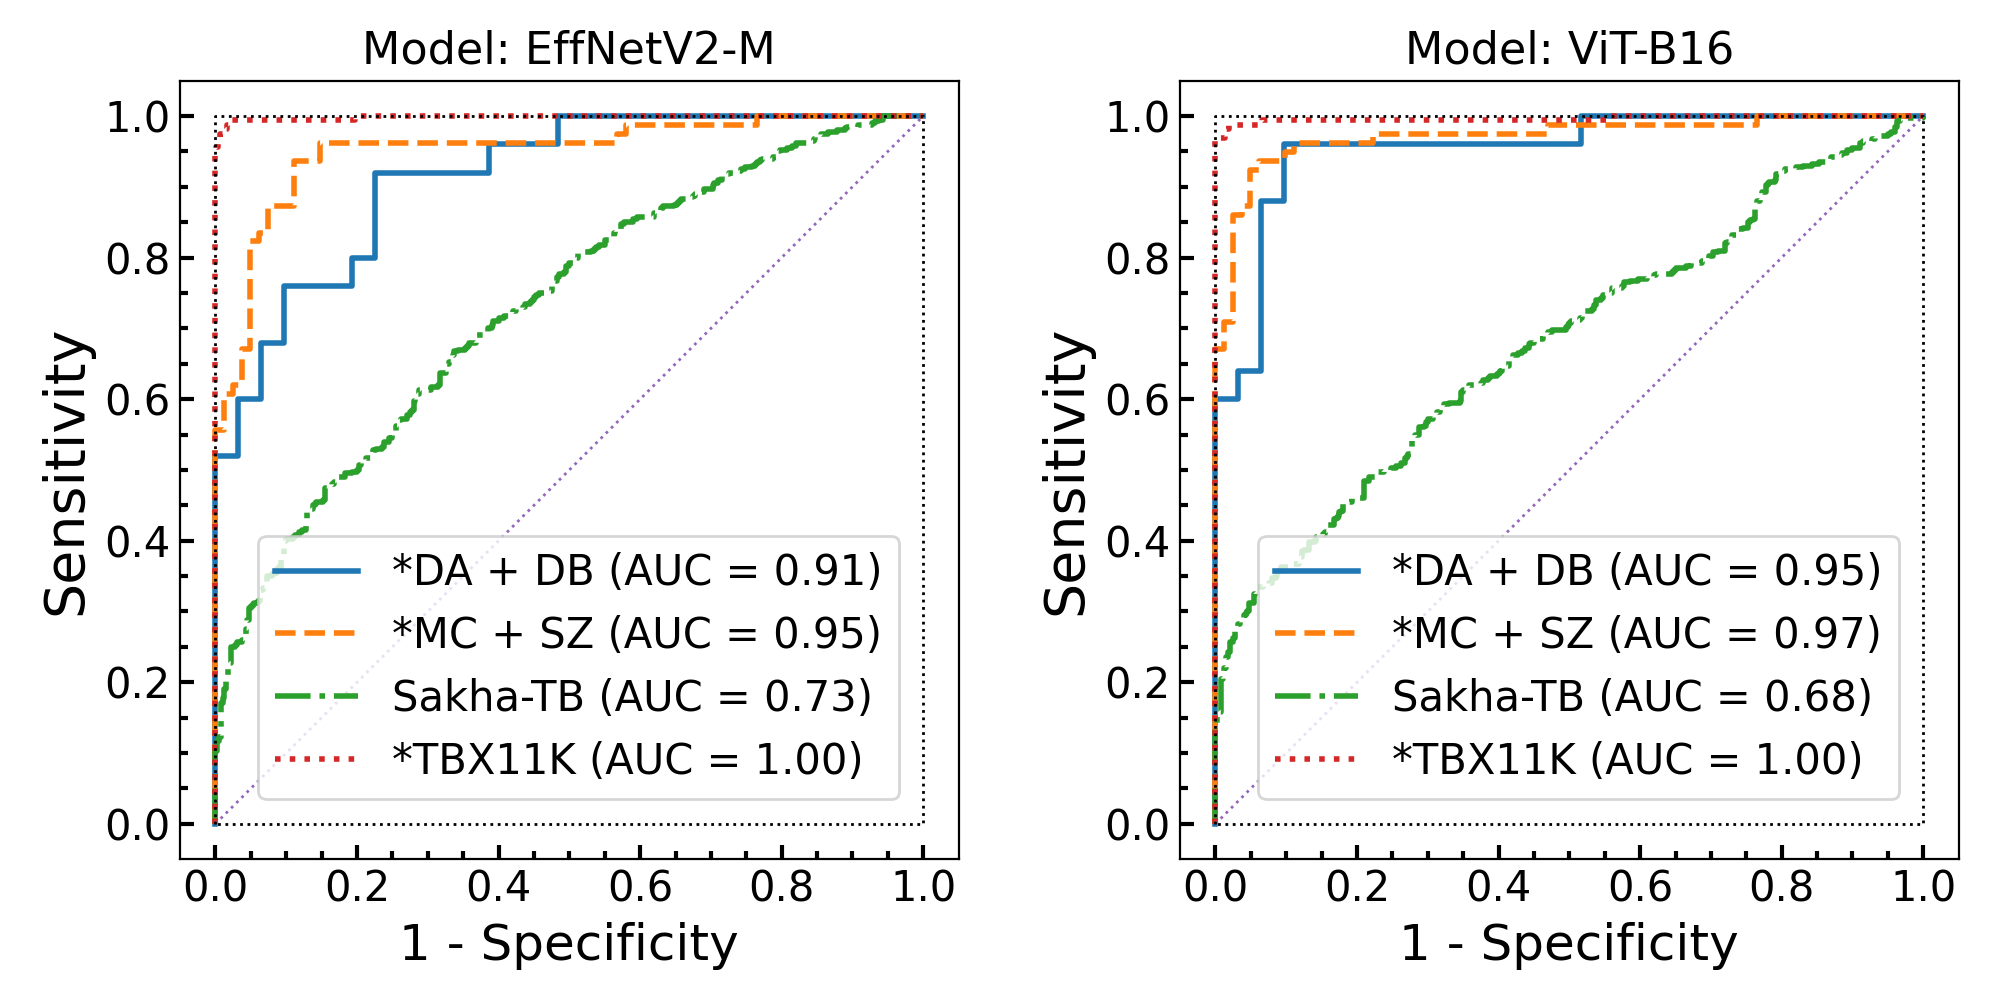
\includegraphics[width=0.9\textwidth]{roc-tbx11k-mc-sz-da-db.png}
%	\caption{Графики ROC"~кривых для моделей, обученных на наборе TBX11K~+~(MC~+~SZ)~+~(DA~+~DB)}\label{fig-roc-tbx11k-mc-sz-da-db}
%\end{figure}

%\begin{figure}[ht]%
%	\centering
%	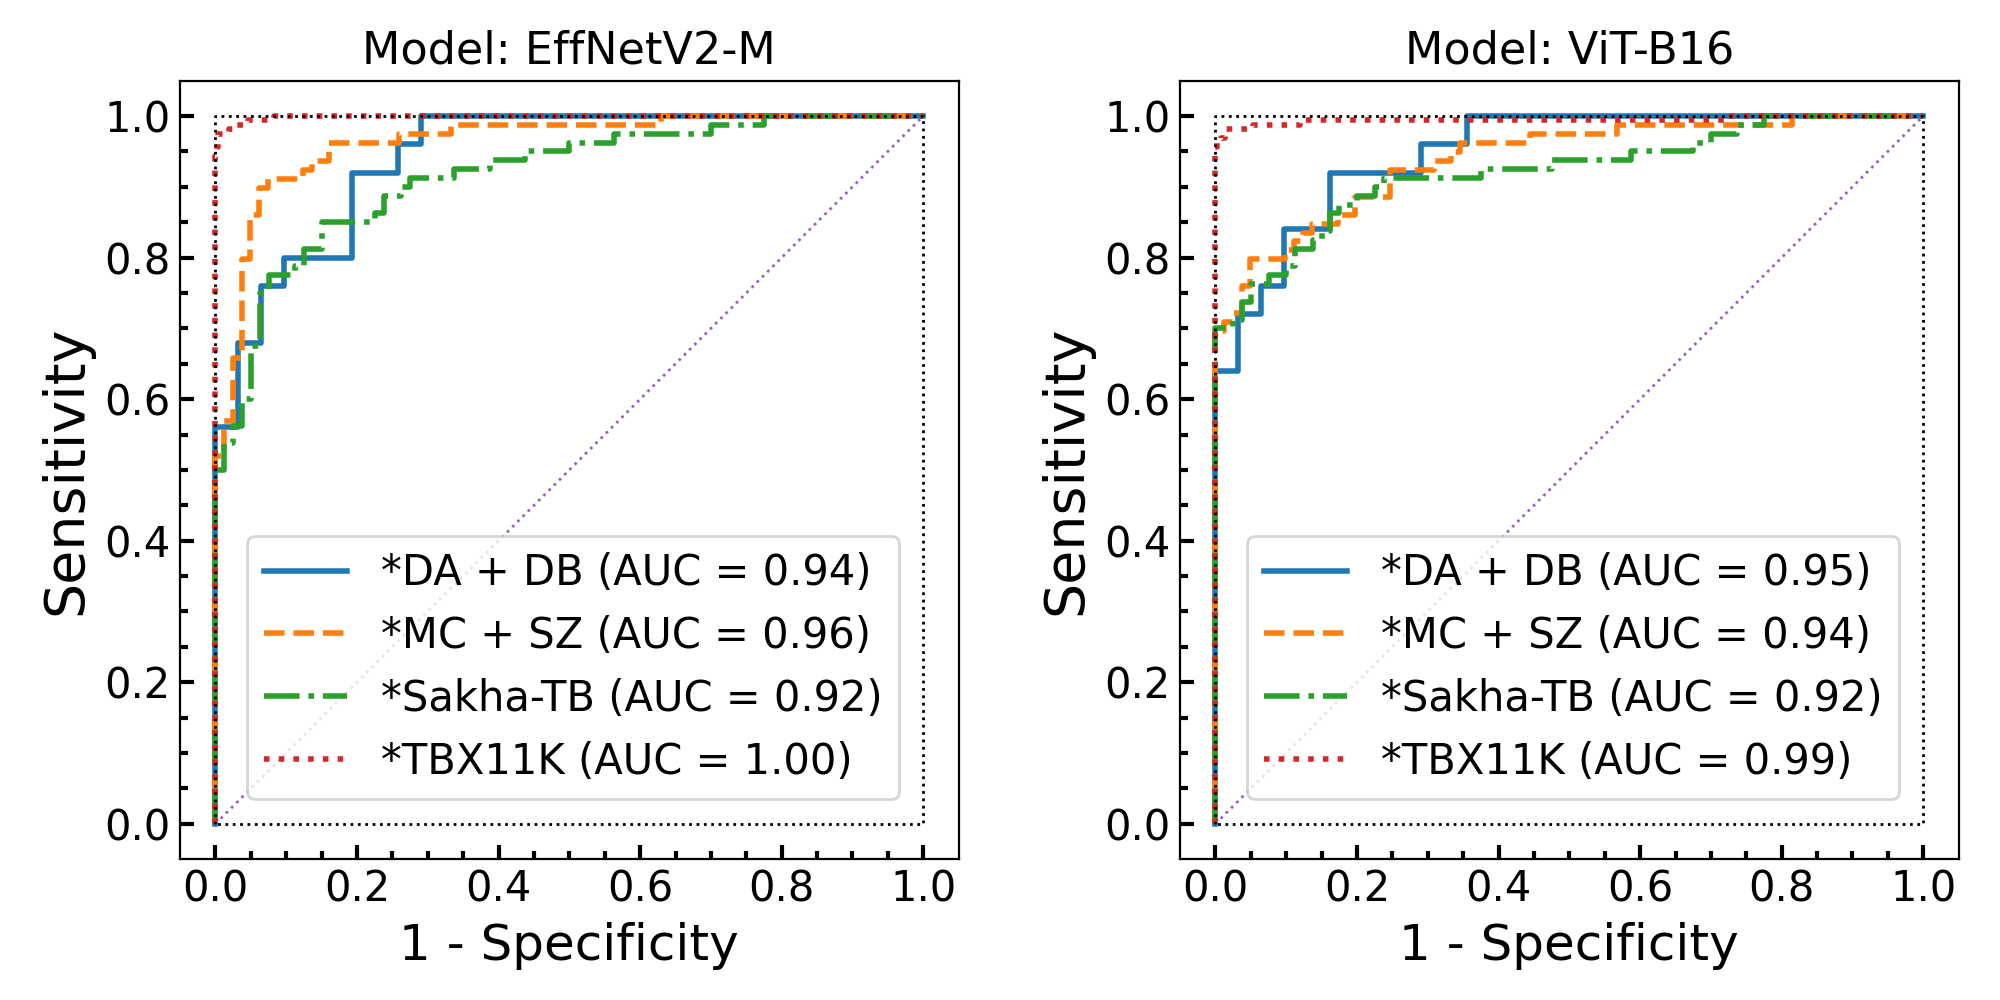
\includegraphics[width=0.9\textwidth]{roc-tbx11k-mc-sz-da-db-sakha.png}
%	\caption{Графики ROC"~кривых для моделей, обученных на наборе TBX11K~+~(MC~+~SZ)~+~(DA~+~DB)~+~Sakha"~TB}\label{fig-roc-tbx11k-mc-sz-da-db-sakha}
%\end{figure}

%Хотя результаты могут значительно различаться в зависимости от использованного алгоритма классификации, на основании графиков и значений меры ROC~AUC на Рис.~\ref{fig-roc-mc-sz}--\ref{fig-roc-sakha} можно сделать вывод, что среди базовых наборов изображений наиболее <<представительным>> являлся MC~+~SZ, так как позволил достичь более высокого качества работы на остальных наборах и в том числе на предлагаемом наборе (лучшее значение ROC~AUC среди двух моделей "--- не ниже 0.85). В то же время TBX11K слабо подготовил алгоритм к работе на данных, отличных от подобных ему. Сформированный в рамках исследования набор проявил себя лучше, чем DA~+~DB, но хуже, чем MC~+~SZ.

%Комбинации двух наборов изображений во время обучения позволили в некоторой степени закрыть <<пробелы>> каждого из наборов, как видно на Рис.~\ref{fig-roc-mc-sz-sakha}--\ref{fig-roc-tbx11k-mc-sz}. Лучше всего себя показала комбинация среднего по размеру MC~+~SZ с предлагаемым Sakha"~TB, позволяя нейросетевому алгоритму почти в равной степени хорошо работать на всех всех четырёх базовых наборах; а сочетание TBX11K и MC~+~SZ всё так же плохо диагностировало заболевание на оставшихся двух наборах, вероятно, из-за дисбаланса в размерах обеих компонент комбинации.

%Объединение всех трёх открытых наборов также не позволило достичь высокого качества диагностики на предлагаемых данных (см.~Рис.~\ref{fig-roc-tbx11k-mc-sz-da-db}).

%Ожидаемо лучше всех себя показало объединение всех 4 базовых наборов (см.~Рис.~\ref{fig-roc-tbx11k-mc-sz-da-db-sakha}).

%Таким образом, эксперименты показали, что лишь добавление предлагаемого набора Sakha"~TB в обучающую выборку и с некоторым допущением самостоятельное использование набора MC~+~SZ дают стабильно высокое качество классификации обученным алгоритмом изображений из всех четырёх рассмотренных наборов рентгеновских снимков. При этом в случае использования представленного набора в качестве основы обучающей выборки не обязательно требуется большой набор изображений. Таким образом, представляется полезным включение набора Sakha"~TB в обучающую выборку нейросетевых моделей компьютерной диагностики туберкулёза для повышения стабильности их работы на практике.

Из графиков видно, что добавление набора Sakha"~TB в обучающую выборку повышает качество работы алгоритма диагностики в том числе на других наборах. При этом в случае использования представленного набора в качестве основы обучающей выборки не обязательно требуется большой набор изображений: комбинация его с набором MC~+~SZ позволила достичь высокого качества диагностики. Таким образом, представляется полезным включение набора Sakha"~TB в обучающую выборку нейросетевых моделей компьютерной диагностики туберкулёза для повышения стабильности их работы на практике.

\clearpage